% Options for packages loaded elsewhere
\PassOptionsToPackage{unicode}{hyperref}
\PassOptionsToPackage{hyphens}{url}
\documentclass[
]{book}
\usepackage{xcolor}
\usepackage{amsmath,amssymb}
\setcounter{secnumdepth}{5}
\usepackage{iftex}
\ifPDFTeX
  \usepackage[T1]{fontenc}
  \usepackage[utf8]{inputenc}
  \usepackage{textcomp} % provide euro and other symbols
\else % if luatex or xetex
  \usepackage{unicode-math} % this also loads fontspec
  \defaultfontfeatures{Scale=MatchLowercase}
  \defaultfontfeatures[\rmfamily]{Ligatures=TeX,Scale=1}
\fi
\usepackage{lmodern}
\ifPDFTeX\else
  % xetex/luatex font selection
\fi
% Use upquote if available, for straight quotes in verbatim environments
\IfFileExists{upquote.sty}{\usepackage{upquote}}{}
\IfFileExists{microtype.sty}{% use microtype if available
  \usepackage[]{microtype}
  \UseMicrotypeSet[protrusion]{basicmath} % disable protrusion for tt fonts
}{}
\makeatletter
\@ifundefined{KOMAClassName}{% if non-KOMA class
  \IfFileExists{parskip.sty}{%
    \usepackage{parskip}
  }{% else
    \setlength{\parindent}{0pt}
    \setlength{\parskip}{6pt plus 2pt minus 1pt}}
}{% if KOMA class
  \KOMAoptions{parskip=half}}
\makeatother
\usepackage{color}
\usepackage{fancyvrb}
\newcommand{\VerbBar}{|}
\newcommand{\VERB}{\Verb[commandchars=\\\{\}]}
\DefineVerbatimEnvironment{Highlighting}{Verbatim}{commandchars=\\\{\}}
% Add ',fontsize=\small' for more characters per line
\usepackage{framed}
\definecolor{shadecolor}{RGB}{248,248,248}
\newenvironment{Shaded}{\begin{snugshade}}{\end{snugshade}}
\newcommand{\AlertTok}[1]{\textcolor[rgb]{0.94,0.16,0.16}{#1}}
\newcommand{\AnnotationTok}[1]{\textcolor[rgb]{0.56,0.35,0.01}{\textbf{\textit{#1}}}}
\newcommand{\AttributeTok}[1]{\textcolor[rgb]{0.13,0.29,0.53}{#1}}
\newcommand{\BaseNTok}[1]{\textcolor[rgb]{0.00,0.00,0.81}{#1}}
\newcommand{\BuiltInTok}[1]{#1}
\newcommand{\CharTok}[1]{\textcolor[rgb]{0.31,0.60,0.02}{#1}}
\newcommand{\CommentTok}[1]{\textcolor[rgb]{0.56,0.35,0.01}{\textit{#1}}}
\newcommand{\CommentVarTok}[1]{\textcolor[rgb]{0.56,0.35,0.01}{\textbf{\textit{#1}}}}
\newcommand{\ConstantTok}[1]{\textcolor[rgb]{0.56,0.35,0.01}{#1}}
\newcommand{\ControlFlowTok}[1]{\textcolor[rgb]{0.13,0.29,0.53}{\textbf{#1}}}
\newcommand{\DataTypeTok}[1]{\textcolor[rgb]{0.13,0.29,0.53}{#1}}
\newcommand{\DecValTok}[1]{\textcolor[rgb]{0.00,0.00,0.81}{#1}}
\newcommand{\DocumentationTok}[1]{\textcolor[rgb]{0.56,0.35,0.01}{\textbf{\textit{#1}}}}
\newcommand{\ErrorTok}[1]{\textcolor[rgb]{0.64,0.00,0.00}{\textbf{#1}}}
\newcommand{\ExtensionTok}[1]{#1}
\newcommand{\FloatTok}[1]{\textcolor[rgb]{0.00,0.00,0.81}{#1}}
\newcommand{\FunctionTok}[1]{\textcolor[rgb]{0.13,0.29,0.53}{\textbf{#1}}}
\newcommand{\ImportTok}[1]{#1}
\newcommand{\InformationTok}[1]{\textcolor[rgb]{0.56,0.35,0.01}{\textbf{\textit{#1}}}}
\newcommand{\KeywordTok}[1]{\textcolor[rgb]{0.13,0.29,0.53}{\textbf{#1}}}
\newcommand{\NormalTok}[1]{#1}
\newcommand{\OperatorTok}[1]{\textcolor[rgb]{0.81,0.36,0.00}{\textbf{#1}}}
\newcommand{\OtherTok}[1]{\textcolor[rgb]{0.56,0.35,0.01}{#1}}
\newcommand{\PreprocessorTok}[1]{\textcolor[rgb]{0.56,0.35,0.01}{\textit{#1}}}
\newcommand{\RegionMarkerTok}[1]{#1}
\newcommand{\SpecialCharTok}[1]{\textcolor[rgb]{0.81,0.36,0.00}{\textbf{#1}}}
\newcommand{\SpecialStringTok}[1]{\textcolor[rgb]{0.31,0.60,0.02}{#1}}
\newcommand{\StringTok}[1]{\textcolor[rgb]{0.31,0.60,0.02}{#1}}
\newcommand{\VariableTok}[1]{\textcolor[rgb]{0.00,0.00,0.00}{#1}}
\newcommand{\VerbatimStringTok}[1]{\textcolor[rgb]{0.31,0.60,0.02}{#1}}
\newcommand{\WarningTok}[1]{\textcolor[rgb]{0.56,0.35,0.01}{\textbf{\textit{#1}}}}
\usepackage{longtable,booktabs,array}
\usepackage{calc} % for calculating minipage widths
% Correct order of tables after \paragraph or \subparagraph
\usepackage{etoolbox}
\makeatletter
\patchcmd\longtable{\par}{\if@noskipsec\mbox{}\fi\par}{}{}
\makeatother
% Allow footnotes in longtable head/foot
\IfFileExists{footnotehyper.sty}{\usepackage{footnotehyper}}{\usepackage{footnote}}
\makesavenoteenv{longtable}
\usepackage{graphicx}
\makeatletter
\newsavebox\pandoc@box
\newcommand*\pandocbounded[1]{% scales image to fit in text height/width
  \sbox\pandoc@box{#1}%
  \Gscale@div\@tempa{\textheight}{\dimexpr\ht\pandoc@box+\dp\pandoc@box\relax}%
  \Gscale@div\@tempb{\linewidth}{\wd\pandoc@box}%
  \ifdim\@tempb\p@<\@tempa\p@\let\@tempa\@tempb\fi% select the smaller of both
  \ifdim\@tempa\p@<\p@\scalebox{\@tempa}{\usebox\pandoc@box}%
  \else\usebox{\pandoc@box}%
  \fi%
}
% Set default figure placement to htbp
\def\fps@figure{htbp}
\makeatother
\setlength{\emergencystretch}{3em} % prevent overfull lines
\providecommand{\tightlist}{%
  \setlength{\itemsep}{0pt}\setlength{\parskip}{0pt}}
\usepackage[]{natbib}
\bibliographystyle{apalike}
\usepackage{booktabs}
\usepackage{amsthm}
\makeatletter
\def\thm@space@setup{%
  \thm@preskip=8pt plus 2pt minus 4pt
  \thm@postskip=\thm@preskip
}
\makeatother
\usepackage{bookmark}
\IfFileExists{xurl.sty}{\usepackage{xurl}}{} % add URL line breaks if available
\urlstyle{same}
\hypersetup{
  pdftitle={Quantitive Methods 2, ZHAW},
  pdfauthor={Jürgen Degenfellner},
  hidelinks,
  pdfcreator={LaTeX via pandoc}}

\title{Quantitive Methods 2, ZHAW}
\author{Jürgen Degenfellner}
\date{2025-01-17}

\begin{document}
\maketitle

{
\setcounter{tocdepth}{1}
\tableofcontents
}
\chapter{Introduction}\label{intro0}

This script is a continuation of
\href{https://jdegenfellner.github.io/Script_QM1_ZHAW/}{the first one} for Quantitative Methods 1
at ZHAW.

In the first part, we learned about the basics of probability theory,
descriptive statistics, Bayesian statistics, and hypothesis testing.

In this script, we will dive into the basics of statistical modeling -
a world of aesthetic wonder and surprises.

This script is a first draft as you are the first group to be working with it.

Please feel free to send me suggestions for improvements or corrections.

This \textbf{should be a collaborative effort} and will (hopefully)
never be finished as our insight grows over time.

The script can also be seen as a pointer to great sources which are
fit to deepen your understanding of the topics. Knowledge is decentralized,
and there are many great ressources out there.

For the working setup with R, please
see \href{https://jdegenfellner.github.io/Script_QM1_ZHAW/index.html\#section}{this}
and the following sections in the first script.

The complete code for this script can be found
\href{https://github.com/jdegenfellner/Script_QM2_ZHAW}{here}.

\section{Books we will heavily borrow from are:}\label{books-we-will-heavily-borrow-from-are}

\begin{itemize}
\tightlist
\item
  (Free) \href{https://civil.colorado.edu/~balajir/CVEN6833/bayes-resources/RM-StatRethink-Bayes.pdf}{Statistical Rethinking}, YouTube-Playlist: \href{https://youtu.be/FdnMWdICdRs?si=q2py5QVY_L299hEa}{Statistical Rethinking 2023}
\item
  (Free) \href{https://vdoc.pub/documents/understanding-regression-analysis-a-conditional-distribution-approach-84oqjr8sqva0}{Understanding Regression Analysis: A Conditional Distribution Approach}
\item
  \href{http://www.stat.columbia.edu/~gelman/arm/}{Data Analysis Using Regression and Multilevel/Hierarchical Models}
\item
  (Free) \href{https://nyu-cdsc.github.io/learningr/assets/kruschke_bayesian_in_R.pdf}{Doing Bayesian Data Analysis}
\end{itemize}

\chapter{Introduction}\label{intro}

\section{What is statistical modeling and what do we need this for?}\label{what-is-statistical-modeling-and-what-do-we-need-this-for}

Typically, one simplifies the complex reality (and loses information) in order to make it better
understandable, mathematically treatable and to make predictions.

Underlying our models, there are theories which should be \href{https://en.wikipedia.org/wiki/Falsifiability}{falsifiable}
and testable.
For instance, I would be really surprised if I pull up my multimeter and measure the voltage (V) and
electric current (I) at a resistence (R) in a circuit and find that \href{https://en.wikipedia.org/wiki/Ohm\%27s_law}{Ohm's law} \(V = IR\) is not true.
This \href{https://en.wikipedia.org/wiki/Scientific_law}{\textbf{law}}
can be tested over and over again and if one would find a single valid counterexample,
the law would be falsified. It is also true that the law is probably not 100\% accularate,
but an extremely good approximation of reality. Real-world measurements carry
measurement errors and when plotting the data, one would see that the data points
might not lie exactly on a straight line. This is not a problem.

A \href{https://en.wikipedia.org/wiki/Statistical_model}{statistical model}
is a mathematical framework that represents the
relationships between variables, helping us understand, infer, and
predict patterns in data. It acts as a bridge between observed data
and the real-world processes that generated them. In health research,
where variability and uncertainty are inherent, statistical models are
valuable tools for making sense of complex phenomena.
You can watch \href{https://www.youtube.com/watch?v=3d5ivs_8amQ&ab_channel=VeryNormal}{this} as short intro.

Depending on the task at hand, we would use different models.
In any case, logical reasoning and critical thinking comes first,
then comes the model. \textbf{It makes no sense to estimate statistical models just for the sake of it}.

\textbf{All models are wrong, but some are useful}.
Or to quote \href{https://www.tandfonline.com/doi/abs/10.1080/01621459.1976.10480949}{George Box}:

\begin{quote}
``Since all models are wrong the scientist cannot obtain
a `correct' one by excessive elaboration. On the contrary
following William of Occam he should seek an economical
description of natural phenomena. Just as the ability to
devise simple but evocative models is the signature of the
great scientist so overelaboration and overparameterization is often the mark of mediocrity.''
\end{quote}

In my opinion, statistical modeling is an art form: difficult and beautiful.

\textbf{One goal of this course} is to improve interpretation and limitations of statistical models.
They are not magical turning data into truth. Firstly, the rule gargabe in, garbage out (GABA) applies.
Secondly, statistical models are based on data and their variability and have inherent limitations
one cannot overcome even with the most sophisticated models. This is expressed for instance
in the so-called \href{https://en.wikipedia.org/wiki/Bias\%E2\%80\%93variance_tradeoff}{bias-variance trade-off}.
You can't have it all.

\subsection{Explanatory vs.~Predictive Models}\label{explanatory-vs.-predictive-models}

I can recommend reading \href{https://projecteuclid.org/journals/statistical-science/volume-25/issue-3/To-Explain-or-to-Predict/10.1214/10-STS330.full}{this}
article by Shmueli et al.~(2010) on this topic.

Statistical models serve different purposes depending on the research question. Two primary goals are \textbf{explanation}
and \textbf{prediction}, and each requires a different approach:

\textbf{Explanatory Models} focus on understanding causal relationships.
These models aim to uncover mechanisms and answer \textbf{``why''}
questions. For example:

\begin{itemize}
\tightlist
\item
  Does smoking increase the risk of lung cancer? \textbf{Yes}. (If you want to see what a large effect-size looks like, check out \href{https://bmjopen.bmj.com/content/bmjopen/8/10/e021611.full.pdf}{this study}.)
\item
  How large is the ``effect'' of smoking on lung cancer? \textbf{Large}.
\item
  Does pain education and graded sensorimotor relearning improve disability (a question we ask in
  our \href{https://data.snf.ch/grants/grant/220585}{Resolve Swiss project})?
\end{itemize}

Explanatory models are \textbf{theory-driven}, designed to test hypotheses. Here, one wants to understand the underlying
mechanisms and the relationships between variables and hence often uses (parsimonious) models that are more interpretable,
like linear regression.

\textbf{Predictive Models} prioritize forecasting future outcomes based on patterns in the data.
These models aim to answer \textbf{``what will happen?''} For instance:

\begin{itemize}
\tightlist
\item
  \href{https://www.tandfonline.com/doi/abs/10.1080/03091902.2020.1822940}{Gait analysis} using Machine Learning (ML)?
\item
  \href{https://jamanetwork.com/journals/jamadermatology/fullarticle/2756346}{Skin cancer detection} using neural networks?
\end{itemize}

Predictive models are \textbf{data-driven}, often using complex algorithms to achieve high accuracy.
Their success is measured using metrics like \href{https://computersciencewiki.org/index.php/Root-mean-square_error_(RMSE)}{Root Means Square Error}
(RMSE), \href{https://en.wikipedia.org/wiki/Receiver_operating_characteristic\#:~:text=The\%20area\%20under\%20the\%20curve,ranks\%20higher\%20than\%20'negative'}{Area Unter the Curve}
(AUC), or \textbf{prediction error on new, unseen data}.
Any amount of model complexity is allowed. One could for instance estimate a
\href{https://en.wikipedia.org/wiki/Neural_network_(machine_learning)}{neural network} (``just'' another statistical model)
with many hidden layers and neurons in order to improve prediction quality. Interpretability of the model weights is not a priority here.

While explanatory and predictive goals often complement each other,
their differences highlight the importance of clearly defining the purpose
of your analysis. In applied health research, explanatory models help identify
causal mechanisms, while predictive models can guide real-world decisions by
providing actionable forecasts. Together, they enhance both our understanding
of phenomena and our ability to make informed decisions in complex environments.

\subsection{Individual vs.~Population Prediction}\label{individual-vs.-population-prediction}

Another important distinction is between \textbf{individual vs.~population} prediction.
In the smoking example above, we can be very sure about the mean effects that smoking has on lung cancer.
On an individual level, it is \href{https://www.liebertpub.com/doi/10.1089/rej.2019.2298}{harder to predict the outcome}.
Nevertheless, individual predictions will be (notably) better than random guessing. We will discuss this in greater detail.

\subsection{Practical Use of Statistical Models}\label{practical-use-of-statistical-models}

In my optinion, we should never be afraid to test our statistical models (as honestly as possible) against reality.
We could for instance ask ourselves:

\begin{itemize}
\item
  ``How much better does this model classify than the arithmetic mean?
  (i.e., the linear model with just an intercept)''
\item
  ``How much better does this model classify than random guessing?''
\item
  Is it worth the effort to collect data and estimate this model by using hundreds of hours of our time?
\end{itemize}

In some cases, these questions can be answered straightforwardly.

\begin{itemize}
\item
  In advertising (Google, Facebook, \ldots), a couple of percentage points in prediction quality might make a difference of millions
  of dollars in revenue offsetting the statistitians salary.
\item
  Improved forecasts of a few percentage points in the stock market or just being \href{https://en.wikipedia.org/wiki/Jim_Simons}{slightly better}
  than the average, will make you faboulously rich.
\item
  Improved cancer forecasting might save lives, money and pain and is not only measured in money.
\end{itemize}

\subsection{Start at the beginning}\label{start-at-the-beginning}

What do we actually want to do in general? Very broadly speaking we want to:
\textbf{describe} the association of variables to each other that carry variability.
Hence, the relationship is not deterministic like \[y = 2x + 3\] but rather we need
to ``loosen up'' the relationship to account for variability (in \(x\) and \(y\)).
So, the values \(2\) and \(3\) are not fixed but aflicted with uncertainty.
Depending on your philosophical view, you might say you want to find
the ``true'' but unknown relationship between variables.
This is what we do in simulation studies all the time: We know the true relationship,
simulate data by adding variability and then try to estimate the true relationship we assumed in the first place.
For some practical applications, we can get a really nice and complete answer to our question
(for instance sample size for proportions).

So we are looking for a function \(f\) such that

\[ Y = f(X) \]

where

\begin{itemize}
\tightlist
\item
  \(Y\) is the ``outcome'', ``dependent variable'' or ``response''.
\item
  \(X\) are the ``predictors''. \(X\) can be a single Variable \(x\) or many
  variables \(x_1, x_2, \ldots, x_p\).
\end{itemize}

It is important to be aware of the notation here:
``Predict'' does \textbf{not necessarily} mean that we can predict the value in
the future. It merely means we estimate the value (or mean) of \(Y\) given \(X\).

\begin{itemize}
\tightlist
\item
  This can be done at the same time points, known as \textbf{cross-sectional} analysis (``What is the maximum jumping height
  of a person given their age at a certain point in time, whereas both variables are measured at the same time?'');
\item
  or at different time points, known as \textbf{longitudinal analysis} (``What is the maximum jumping height of a person 10 years later (\(t_2\))
  given their baseline health status at time \(t_1\)?'').
\end{itemize}

The \textbf{simplest statistical model} would be the mean model where \(Y\) is ``predicted'' by a
constant: \(Y = c\) which (at least in the classical linear regression) turns out to be \(c = \bar{x}\).
This simple model is often surprisingly good, or, to put it in other words, models with more complexity
are often not that much better with regards to multiple metrics.

\section{A (simple) model for adult body heights in the Bayesian framework}\label{a-simple-model-for-adult-body-heights-in-the-bayesian-framework}

As repetition, read the parts about \href{https://jdegenfellner.github.io/Script_QM1_ZHAW/bayes_statistics.html}{Bayes statistics from QM1}
again to refresh your memory about the Bayesian framework.

It's recommendable to read the beginning of the book \href{https://civil.colorado.edu/~balajir/CVEN6833/bayes-resources/RM-StatRethink-Bayes.pdf}{Statistical rethinking}
up until page 39 as well. We are not completely new to the topic of Bayes due
to QM1.

We want to \textbf{start building our first model} right away.

Let's begin with the example in
\href{https://civil.colorado.edu/~balajir/CVEN6833/bayes-resources/RM-StatRethink-Bayes.pdf}{Statistical rethinking}
using data from the \href{https://en.wikipedia.org/wiki/\%C7\%83Kung_people}{!Kung San}
people starting on page 79.

\begin{Shaded}
\begin{Highlighting}[]
\FunctionTok{library}\NormalTok{(rethinking)}
\FunctionTok{data}\NormalTok{(}\StringTok{"Howell1"}\NormalTok{)}
\NormalTok{d }\OtherTok{\textless{}{-}}\NormalTok{ Howell1}
\FunctionTok{str}\NormalTok{(d)}
\end{Highlighting}
\end{Shaded}

\begin{verbatim}
## 'data.frame':    544 obs. of  4 variables:
##  $ height: num  152 140 137 157 145 ...
##  $ weight: num  47.8 36.5 31.9 53 41.3 ...
##  $ age   : num  63 63 65 41 51 35 32 27 19 54 ...
##  $ male  : int  1 0 0 1 0 1 0 1 0 1 ...
\end{verbatim}

\begin{Shaded}
\begin{Highlighting}[]
\NormalTok{d2 }\OtherTok{\textless{}{-}}\NormalTok{ d[d}\SpecialCharTok{$}\NormalTok{age }\SpecialCharTok{\textgreater{}=} \DecValTok{18}\NormalTok{, ] }\CommentTok{\# only adults}
\end{Highlighting}
\end{Shaded}

We want to model the adult height of the !Kun San people
using prior knowledge (about the Swiss population) and data.

\begin{Shaded}
\begin{Highlighting}[]
\FunctionTok{library}\NormalTok{(tidyverse)}
\NormalTok{d2 }\SpecialCharTok{\%\textgreater{}\%} \FunctionTok{ggplot}\NormalTok{(}\FunctionTok{aes}\NormalTok{(}\AttributeTok{x =}\NormalTok{ height)) }\SpecialCharTok{+} \FunctionTok{geom\_histogram}\NormalTok{()}
\end{Highlighting}
\end{Shaded}

\pandocbounded{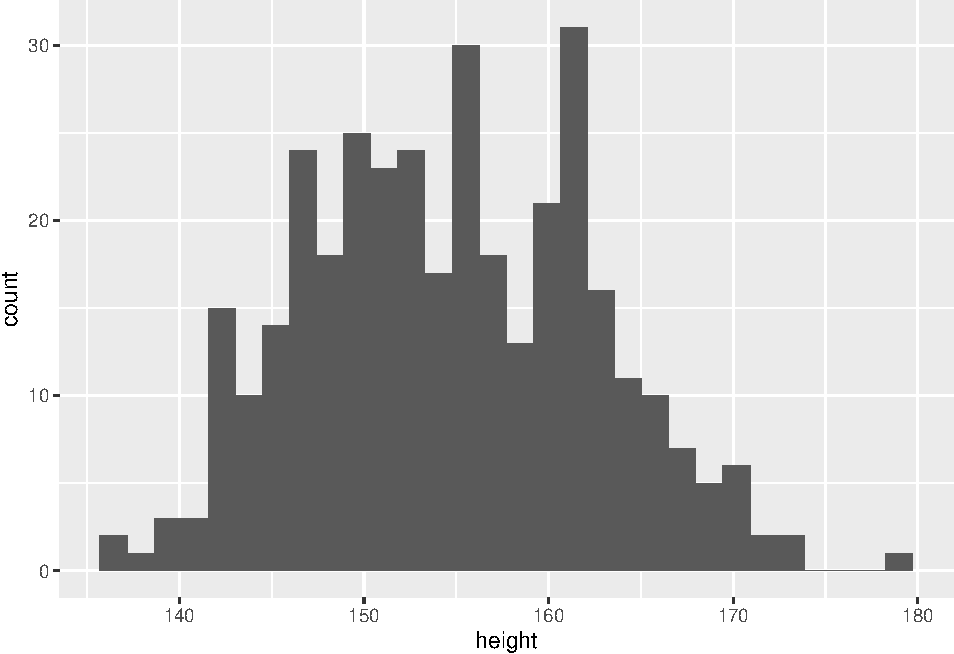
\includegraphics[keepaspectratio]{bookdown-demo_files/figure-latex/unnamed-chunk-2-1.pdf}}

Since we already have domain knowledge in this area, we can say that heights are usually normally distributed,
or at least a mixture of normal distrubutions (female/male).
We assume the following model:
\[h_i \sim \text{Normal}(\mu, \sigma)\]

As in \href{https://jdegenfellner.github.io/Script_QM1_ZHAW/}{QM1},
we want to start with a Bayesian model and hence, we need some priors.

Since we are in Switzerland and just for fun, we use the mean of
\href{https://www.bfs.admin.ch/asset/de/30305714}{Swiss body heights}
as expected value for the \textbf{prior for the mean}.
According to the link (Bundesamt für Statistik),
the mean height of \(n=21,873\) people in the Swiss sample is
\(171.1\) cm. We choose the same \(\sigma\) for the prior of the normal
as in the book not to deviate too much from the example at hand.

Next comes our \textbf{model definition in the Bayesian framework}, which
I often find more intuitive than the frequentist approach:

\[
h_i \sim \text{Normal}(\mu, \sigma)
\]
\[
\mu \sim \text{Normal}(171.1, 20)
\]
\[
\sigma \sim \text{Uniform}(0, 50)
\]

\textbf{Description of the model definition}: The heights are normally distributed with unknown mean and
standard deviation. As our current knowledge about the mean height, we use
a prior distribution for the mean (we do not know but want to estimate) by
assuming the mean of a population we know and a standard deviation of \(20\) cm which
allows are rather large range of possible values for \(\mu\).
\(\sigma\) is also unknown and a priori we restrict ourselves to values
between \(0\) and \(50\) cm, whereas we assign equal plausibility to all
values in this range (which can and should be critically discussed).

\textbf{Vizualisation of the model structure}:
\pandocbounded{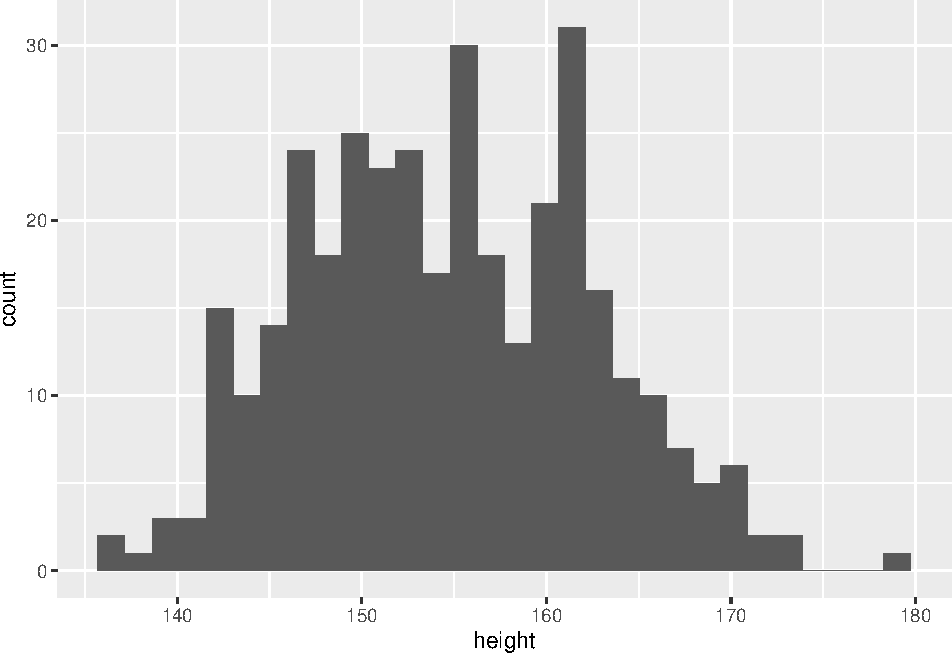
\includegraphics[keepaspectratio]{bookdown-demo_files/figure-latex/unnamed-chunk-3-1.pdf}}

Mind that there is a conceptual difference between the normal distribution of the heights
and the normal prior distribution of the mean. The latter expresses our prior knowledge/insecurity
about the unobserved mean. The normal distribution says we expect the heights to be normally distributed
but we do not know the parameters (\(\mu\) and \(\sigma\)) yet.

Of course we would not need the prior here due to the large sample size,
but let's do it anyways for demonstration purposes.
We are not completely uninformed about body heights and express our
knowledge with the prior for \(\mu\).
The \(20\) in the prior for the mean expresses our range of possible true
mean values and aknowledge
that there are a variety of different subpopulations with different means.

Using the Swiss data in the link one could estimate that the standard deviation of the heights
from \(21,873\) Swiss people is around is \(25.6553\) cm (\hyperref[exercise1_Intro]{Exercise 1}).

Remember, in the Baysian world, there is no \textbf{fixed but unknown}
parameter, but instead we define a distribution over the unobserved parameter.

We \textbf{visualize the prior for \(\mu\)}.

\begin{Shaded}
\begin{Highlighting}[]
\FunctionTok{curve}\NormalTok{(}\FunctionTok{dnorm}\NormalTok{(x, }\FloatTok{171.1}\NormalTok{, }\DecValTok{20}\NormalTok{), }\AttributeTok{from =} \DecValTok{100}\NormalTok{, }\AttributeTok{to =} \DecValTok{250}\NormalTok{)}
\end{Highlighting}
\end{Shaded}

\pandocbounded{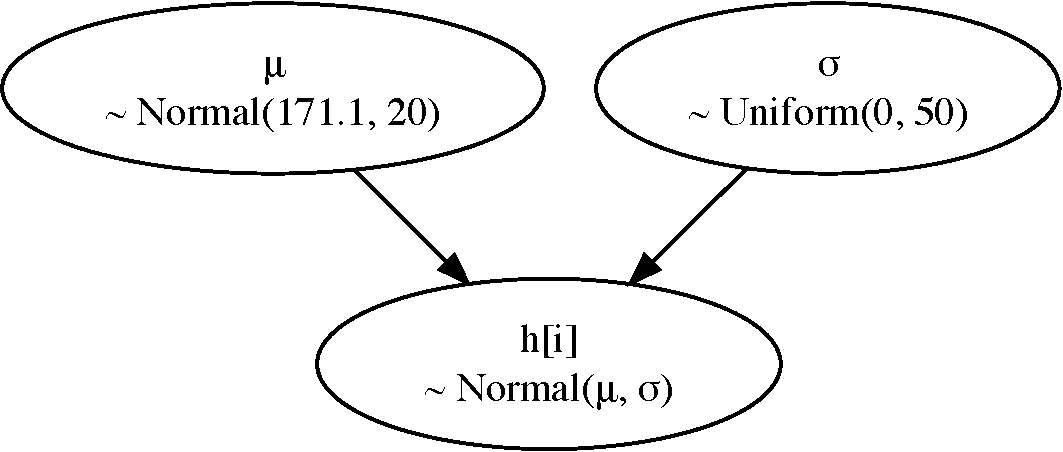
\includegraphics[keepaspectratio]{bookdown-demo_files/figure-latex/unnamed-chunk-4-1.pdf}}

The \textbf{prior for \(\sigma\)} is uniform between \(0\) and \(50\) cm. This is a very wide prior and
just constrains the values to be positive and below \(50\) cm.
This could be stronger of course.

\textbf{Visualization of the prior for \(\sigma\)}:

\begin{Shaded}
\begin{Highlighting}[]
\FunctionTok{curve}\NormalTok{(}\FunctionTok{dunif}\NormalTok{(x, }\DecValTok{0}\NormalTok{, }\DecValTok{50}\NormalTok{), }\AttributeTok{from =} \SpecialCharTok{{-}}\DecValTok{10}\NormalTok{, }\AttributeTok{to =} \DecValTok{60}\NormalTok{)}
\end{Highlighting}
\end{Shaded}

\pandocbounded{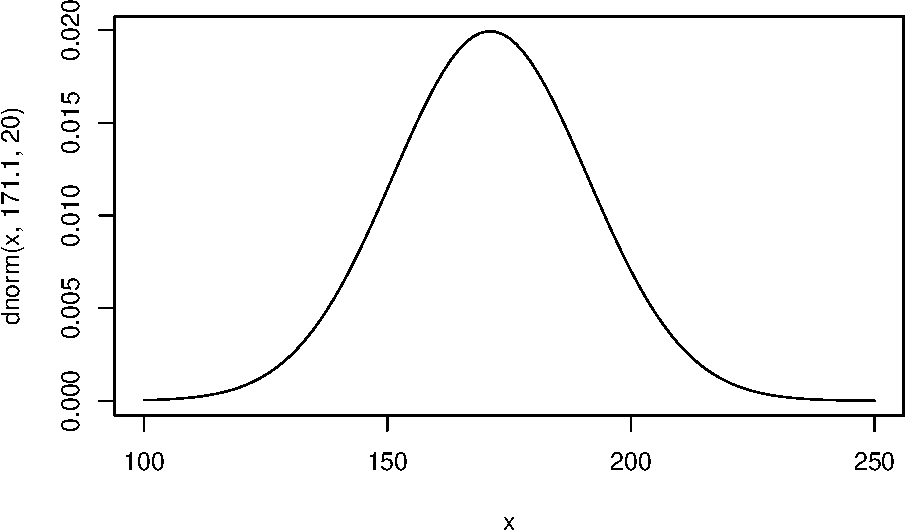
\includegraphics[keepaspectratio]{bookdown-demo_files/figure-latex/unnamed-chunk-5-1.pdf}}

Note, we didn't specify a prior probability distribution of heights
directly, but once we've chosen priors for \(\mu\) and \(\sigma\), these imply a
prior distribution of individual heights.

\textbf{Without} even having seen the \textbf{new data}, we can check what our prior
(model) for heights would predict. This is important. If the prior already
predicts impossible values, we should reconsider our priors and/or model.

So, we simply draw \(\mu\) and \(\sigma\) from the priors and then draw heights
from the normal distribution using the drawn parameters.

\textbf{Vizualisation of the prior for heights}:

\begin{Shaded}
\begin{Highlighting}[]
\NormalTok{sample\_mu }\OtherTok{\textless{}{-}} \FunctionTok{rnorm}\NormalTok{(}\DecValTok{10}\SpecialCharTok{\^{}}\DecValTok{4}\NormalTok{, }\FloatTok{171.1}\NormalTok{, }\DecValTok{20}\NormalTok{)}
\NormalTok{sample\_sigma }\OtherTok{\textless{}{-}} \FunctionTok{runif}\NormalTok{(}\DecValTok{10}\SpecialCharTok{\^{}}\DecValTok{4}\NormalTok{, }\DecValTok{0}\NormalTok{, }\DecValTok{50}\NormalTok{)}
\NormalTok{prior\_h }\OtherTok{\textless{}{-}} \FunctionTok{rnorm}\NormalTok{(}\DecValTok{10}\SpecialCharTok{\^{}}\DecValTok{4}\NormalTok{, sample\_mu, sample\_sigma)}
\FunctionTok{length}\NormalTok{(prior\_h)}
\end{Highlighting}
\end{Shaded}

\begin{verbatim}
## [1] 10000
\end{verbatim}

\begin{Shaded}
\begin{Highlighting}[]
\FunctionTok{dens}\NormalTok{(prior\_h)}
\end{Highlighting}
\end{Shaded}

\pandocbounded{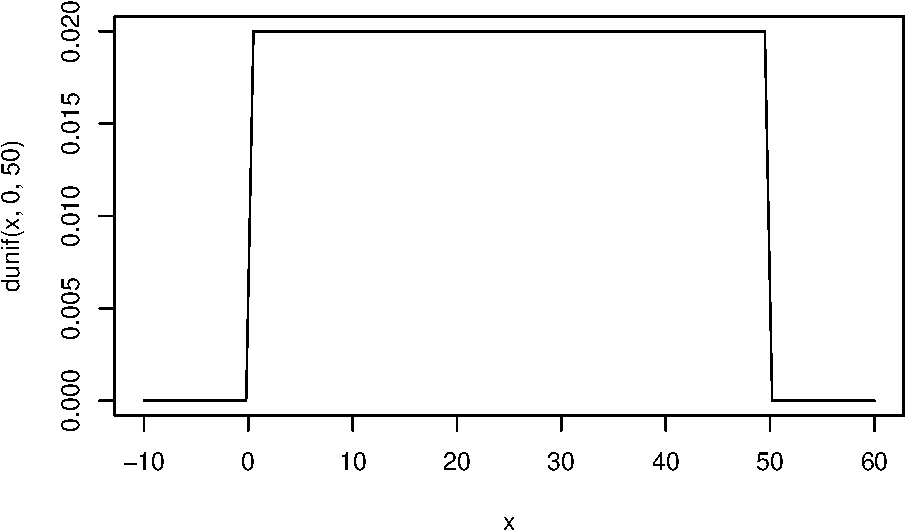
\includegraphics[keepaspectratio]{bookdown-demo_files/figure-latex/unnamed-chunk-6-1.pdf}}

The prior is not itself a Gaussian distribution, but a distribution of
relative plausibilities of different heights, before seeing the data.

Now, there are a couple of different ways to estimtate the model incorporating
the new data. For didactic reasons, grid approximation is often used (as in the book).
For many parameters, grid approximation becomes more and more infeasible (due to combinatorial explosion).

We will skip that for now and use quadratic approximation instead which
works well for many common procedures in applied statistics (like linear regression).
Later, you'll probably use (or the software in the background) mostly Markov
chain Monte Carlo (MCMC) sampling to get the posterior.
\href{https://civil.colorado.edu/~balajir/CVEN6833/bayes-resources/RM-StatRethink-Bayes.pdf}{Pages 39 and the following}
explain the 3 concepts grid approximation, quadratic approximation and MCMC.

In short, \textbf{quadratic approximation} assumes that our posterior distribution
of body heights can be approximated well by a normal distribution,
at least near the peak.

Please read the \hyperref[bivariate_normal]{addendum} to get a clearer picture of
what a bivariate normal distribution is.

Using the library \texttt{rethinking} we can estimate the model using quadratic approximation.
First, we define the model in the \texttt{rethinking} syntax (see R code 4.25 in the book).

\begin{Shaded}
\begin{Highlighting}[]
\FunctionTok{library}\NormalTok{(rethinking)}
\NormalTok{flist }\OtherTok{\textless{}{-}} \FunctionTok{alist}\NormalTok{(}
\NormalTok{  height }\SpecialCharTok{\textasciitilde{}} \FunctionTok{dnorm}\NormalTok{(mu, sigma),}
\NormalTok{  mu }\SpecialCharTok{\textasciitilde{}} \FunctionTok{dnorm}\NormalTok{(}\FloatTok{171.1}\NormalTok{, }\DecValTok{20}\NormalTok{),}
\NormalTok{  sigma }\SpecialCharTok{\textasciitilde{}} \FunctionTok{dunif}\NormalTok{(}\DecValTok{0}\NormalTok{, }\DecValTok{50}\NormalTok{)}
\NormalTok{)}
\end{Highlighting}
\end{Shaded}

Then we estimate/fit the model using quadratic approximation.

\begin{Shaded}
\begin{Highlighting}[]
\NormalTok{m\_heights }\OtherTok{\textless{}{-}} \FunctionTok{quap}\NormalTok{(flist, }\AttributeTok{data =}\NormalTok{ d2)}
\end{Highlighting}
\end{Shaded}

Now let's take a look at the fitted model:
(Note: In the online-version of the book, they used the command \texttt{map} instead of \texttt{quap}.)

\begin{Shaded}
\begin{Highlighting}[]
\FunctionTok{precis}\NormalTok{(m\_heights)}
\end{Highlighting}
\end{Shaded}

\begin{verbatim}
##             mean        sd       5.5%      94.5%
## mu    154.606387 0.4119860 153.947954 155.264820
## sigma   7.731172 0.2913708   7.265505   8.196838
\end{verbatim}

Above, we see the mean of the posterior for \(\mu\) \textbf{and} \(\sigma\);
and a 89\% credible interval for those parameters.

We can now plot the posterior distribution of the mean and the standard deviation.

\begin{Shaded}
\begin{Highlighting}[]
\NormalTok{post }\OtherTok{\textless{}{-}} \FunctionTok{extract.samples}\NormalTok{(m\_heights, }\AttributeTok{n =} \DecValTok{10}\SpecialCharTok{\^{}}\DecValTok{4}\NormalTok{)}
\FunctionTok{head}\NormalTok{(post)}
\end{Highlighting}
\end{Shaded}

\begin{verbatim}
##         mu    sigma
## 1 154.3658 8.455891
## 2 154.3274 7.903180
## 3 154.5510 7.704259
## 4 154.3533 7.778473
## 5 154.2720 8.143232
## 6 154.2503 7.849285
\end{verbatim}

\begin{Shaded}
\begin{Highlighting}[]
\FunctionTok{dens}\NormalTok{(post}\SpecialCharTok{$}\NormalTok{mu)}
\end{Highlighting}
\end{Shaded}

\pandocbounded{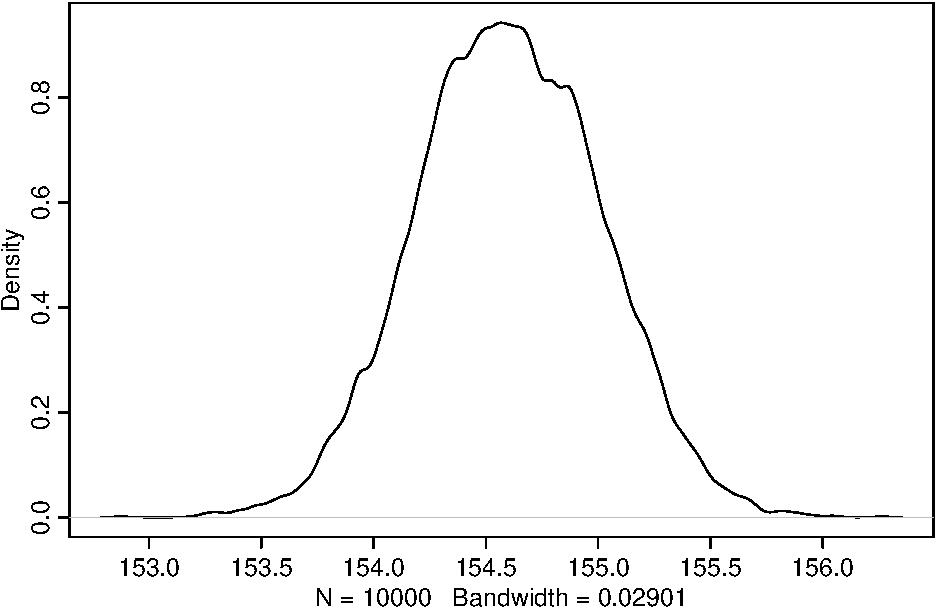
\includegraphics[keepaspectratio]{bookdown-demo_files/figure-latex/unnamed-chunk-10-1.pdf}}

\begin{Shaded}
\begin{Highlighting}[]
\FunctionTok{dens}\NormalTok{(post}\SpecialCharTok{$}\NormalTok{sigma)}
\end{Highlighting}
\end{Shaded}

\pandocbounded{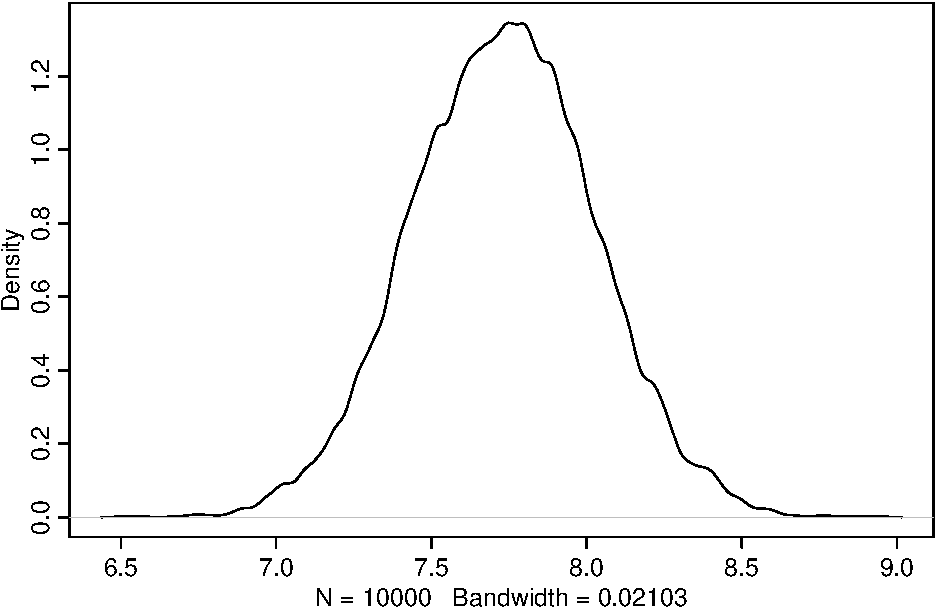
\includegraphics[keepaspectratio]{bookdown-demo_files/figure-latex/unnamed-chunk-10-2.pdf}}

Note, that \textbf{these samples come from a multi-dimensional posterior distribution}.
In our case, we approximated the posterior with a
\href{https://en.wikipedia.org/wiki/Multivariate_normal_distribution}{bivariate normal distribution}.
They are not necessarily independent from each other, but in this case they are.
We know this from the model definition above. \(\mu\) and \(\sigma\) are both
defined as normal respectively uniform distributions and by definition do not
influence each other. This is also visible in the vizualisation of the model structure:
There is no confounding variable or connection between those priors. One could
think of a common variable \(Z\) that influences both \(\mu\) and \(\sigma\). This could
be genetic similarity which could influence both \(\mu\) and \(\sigma\).

Let's verify that \(\mu\) and \(\sigma\) are uncorrelated:

\begin{Shaded}
\begin{Highlighting}[]
\FunctionTok{vcov}\NormalTok{(m\_heights)}
\end{Highlighting}
\end{Shaded}

\begin{verbatim}
##                 mu        sigma
## mu    0.1697324421 0.0002040443
## sigma 0.0002040443 0.0848969479
\end{verbatim}

gives you the variance-covariance matrix of the parameters of the posterior
distribution. In the diagonal you see the variance of the parameters.

\begin{Shaded}
\begin{Highlighting}[]
\FunctionTok{diag}\NormalTok{(}\FunctionTok{vcov}\NormalTok{(m\_heights))}
\end{Highlighting}
\end{Shaded}

\begin{verbatim}
##         mu      sigma 
## 0.16973244 0.08489695
\end{verbatim}

And we can compute the correlation matrix easily:

\begin{Shaded}
\begin{Highlighting}[]
\FunctionTok{cov2cor}\NormalTok{(}\FunctionTok{vcov}\NormalTok{(m\_heights))}
\end{Highlighting}
\end{Shaded}

\begin{verbatim}
##                mu       sigma
## mu    1.000000000 0.001699793
## sigma 0.001699793 1.000000000
\end{verbatim}

Let's plot the posterior in 3D, because we \textbf{can}:

\pandocbounded{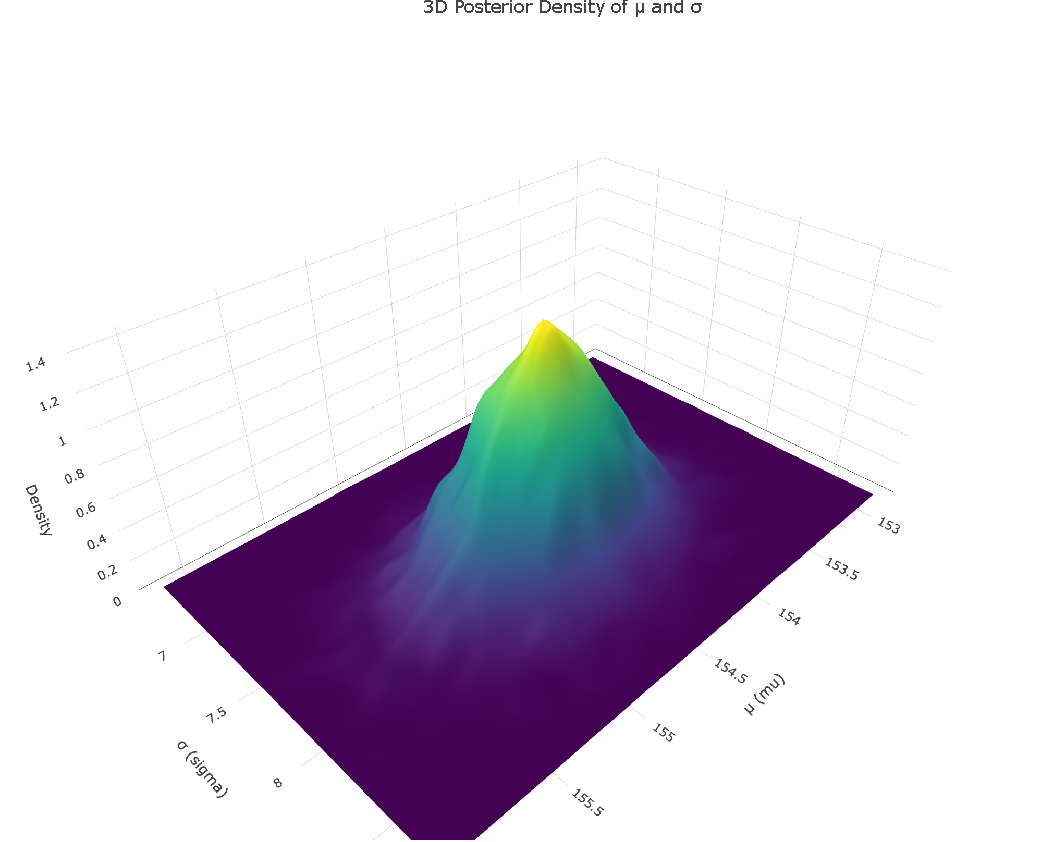
\includegraphics[keepaspectratio]{bookdown-demo_files/figure-latex/posterior-3d-correct-1.pdf}}

\textbf{How beautiful ist that?}

We see in the 3D plot, that the ``mountain'' is not rotated, indicating
graphically that the parameters are independent from each other.

We also see in the correlation matrix, the correlation of the parameters is \(\sim 0\).
In the \href{https://en.wikipedia.org/wiki/Correlation\#Correlation_and_independence}{context of a joint normal distribution},
this means that the parameters are independent.

And, it is not an accident that the posterior looks like this. Using quadratic approximation,
we used the bivariate normal distribution to \textbf{approximate} the posterior.

\section{Classical approach for the simplest model}\label{classical-approach-for-the-simplest-model}

We have seen, how we could use domain and prior knowledge to fit a very simple model
for body heights of a population (!Kung San) in the Bayesian framework.

Now, let's start at the same point in the classical framework.
Here, we do not use any prior knowledge, at least not that explicitely.

The classical approach to fit a regression line is the so-called
\textbf{\href{https://en.wikipedia.org/wiki/Least_squares}{least squares method}}.

The \textbf{(simple mean-) model} is:

\[ Y_i = height_i = c + \varepsilon_i \]

\begin{itemize}
\tightlist
\item
  for some \(c \in \mathbb{R}\) and
\item
  normally distributed errors \(\varepsilon_i \sim \text{Normal}(0, \sigma)\).
\end{itemize}

These are on average zero and have a constant standard deviation of \(\sigma\).
So, we assume there is a fixed, but unknown, constant \(c\) that we want to estimate and we
assume that there is a special sort of error in our model that is normally distributed.
Sometimes there is a large deviation from the true \(c\), sometimes there is a small deviation.
On average, the deviations are zero and the \textbf{errors should also be independent from each other}:
\[ \varepsilon_i \perp \varepsilon_j \text{ for } i \neq j\]
This means that just because I have just observed a large deviation from the true \(c\)
does not mean, that the probability of a large deviation in the next observation is higher/lower.
Note, that we cannot readily define different types of errors in the classical framework.

But what is \(c\)? We determine the shape of the model
ourselves (constant model, or mean model) and then estimate the parameter \(c\).
By defining the shape of the model ourselves and imposing a distribution where we want to
estimate the parameter of said distribution, we are in \textbf{parametric statistics}.

We choose the \(c\) which minimizes the sum of squared errors from the actual heights.
This has the advantage that deviations upper and lower from the actual height are
equally weighted. The larger the deviation the (quadratically) larger the penalty.

\textbf{Why do we do that?} Because, if the model assumptions (more on that later)
are correct, the least squares
estimator is a really good estimator. How good? Later\ldots{}

We want to miminize the following function:

\[ SSE \text{ (Sum of Squared Errors) }(c) = (height_1 - c)^2 + (height_2 - c)^2 + 
\ldots + (height_n - c)^2 =\]
\[ = \sum_{i=1}^{n} (height_i - c)^2\]

The SSE is a function of \(c\) and we want to find the \(c\) that minimizes the function.
Since it is a quadratic function, we can always find the minimum.
We have learnt in school how to do this (hopefully): Take the derivative of the function
and set it to zero. Solve for \(c\) and you have the \(c\) which yields the minimum of SSE(c).

Let's do that:

\[ \frac{d}{dc} SSE(c) =  2(height_1 - c)(-1) + 2(height_2 - c)(-1) + 
\ldots + 2(height_n - c)(-1) =\]
\[ = -2 \sum_{i=1}^{n} (height_i - c)\]

This should be zero for the minimum:
\[ -2 \sum_{i=1}^{n} (height_i - c) = 0\]
\[ \sum_{i=1}^{n} (height_i - c) = 0\]
\[ \sum_{i=1}^{n} (height_i - c) = 0\]
\[ \sum_{i=1}^{n} height_i - n \cdot c = 0\]
\[ \hat{c} = \frac{1}{n} \sum_{i=1}^{n} height_i = \overline{height_i}\]

The hat over the \(c\) indicates that this is the estimated value of \(c\).
Everytime we estimate a parameter, we put a hat over it.

And voilà, we have estimated the parameter \(c\) of the model, which is just the
sample mean of all the heights. In contrast to before, we did not put
in a lot of prior knowledge, but just estimated the parameter from the data.

In R, we can do this easily:

\begin{Shaded}
\begin{Highlighting}[]
\NormalTok{mod }\OtherTok{\textless{}{-}} \FunctionTok{lm}\NormalTok{(height }\SpecialCharTok{\textasciitilde{}} \DecValTok{1}\NormalTok{, }\AttributeTok{data =}\NormalTok{ d2)}
\FunctionTok{summary}\NormalTok{(mod)}
\end{Highlighting}
\end{Shaded}

\begin{verbatim}
## 
## Call:
## lm(formula = height ~ 1, data = d2)
## 
## Residuals:
##      Min       1Q   Median       3Q      Max 
## -18.0721  -6.0071  -0.2921   6.0579  24.4729 
## 
## Coefficients:
##             Estimate Std. Error t value Pr(>|t|)    
## (Intercept) 154.5971     0.4127   374.6   <2e-16 ***
## ---
## Signif. codes:  0 '***' 0.001 '**' 0.01 '*' 0.05 '.' 0.1 ' ' 1
## 
## Residual standard error: 7.742 on 351 degrees of freedom
\end{verbatim}

\begin{Shaded}
\begin{Highlighting}[]
\FunctionTok{dim}\NormalTok{(d2)}
\end{Highlighting}
\end{Shaded}

\begin{verbatim}
## [1] 352   4
\end{verbatim}

\begin{Shaded}
\begin{Highlighting}[]
\FunctionTok{mean}\NormalTok{(d2}\SpecialCharTok{$}\NormalTok{height) }\CommentTok{\# same as the intercept}
\end{Highlighting}
\end{Shaded}

\begin{verbatim}
## [1] 154.5971
\end{verbatim}

\begin{Shaded}
\begin{Highlighting}[]
\FunctionTok{sd}\NormalTok{(d2}\SpecialCharTok{$}\NormalTok{height) }\SpecialCharTok{/} \FunctionTok{sqrt}\NormalTok{(}\FunctionTok{nrow}\NormalTok{(d2)) }\CommentTok{\# standard error of the estimator}
\end{Highlighting}
\end{Shaded}

\begin{verbatim}
## [1] 0.4126677
\end{verbatim}

\begin{Shaded}
\begin{Highlighting}[]
\CommentTok{\# test{-}statistic for the intercept:}
\FunctionTok{mean}\NormalTok{(d2}\SpecialCharTok{$}\NormalTok{height) }\SpecialCharTok{/}\NormalTok{ (}\FunctionTok{sd}\NormalTok{(d2}\SpecialCharTok{$}\NormalTok{height) }\SpecialCharTok{/} \FunctionTok{sqrt}\NormalTok{(}\FunctionTok{nrow}\NormalTok{(d2)))}
\end{Highlighting}
\end{Shaded}

\begin{verbatim}
## [1] 374.6285
\end{verbatim}

\begin{Shaded}
\begin{Highlighting}[]
\CommentTok{\# residual standard error:}
\FunctionTok{sqrt}\NormalTok{(}\FunctionTok{sum}\NormalTok{(mod}\SpecialCharTok{$}\NormalTok{residuals}\SpecialCharTok{\^{}}\DecValTok{2}\NormalTok{) }\SpecialCharTok{/}\NormalTok{ (}\FunctionTok{nrow}\NormalTok{(d2) }\SpecialCharTok{{-}} \DecValTok{1}\NormalTok{))}
\end{Highlighting}
\end{Shaded}

\begin{verbatim}
## [1] 7.742332
\end{verbatim}

the \texttt{\textasciitilde{}1} means that there is just a so-called \textbf{intercept} in the model.
There are \textbf{no covariates}, just the constant \(c\).
This is the simplest we can do. \texttt{lm} stands for linear model and with this base
command in R we ask the software to do the least squares estimation for us.

Let's look at the \textbf{R-output} of the model estimation:

\begin{itemize}
\tightlist
\item
  \texttt{lm(formula\ =\ height\ \textasciitilde{}\ 1,\ data\ =\ d2)}: This is the model we estimated.
\item
  \texttt{Residuals}: The difference between the actual height and the estimated height:
  \(r_i = height_i - \hat{c}\). A univariate 5-point summary is given.
\item
  \texttt{Coefficients}: The estimated coefficients of the model. In this case, there is just the intercept.
  We get the

  \begin{itemize}
  \tightlist
  \item
    \texttt{Std.\ Error} of the estimate, i.e.~the \href{https://en.wikipedia.org/wiki/Standard_error}{standard error} of the mean,
    which is (according to the Central Limit Theorem)
    \[\frac{\sigma}{\sqrt{n}}\] and can be estimated by the sample
    standard deviation divided by the square root of the sample size.
  \item
    the \texttt{t\ value} and the \texttt{Pr(\textgreater{}\textbar{}t\textbar{})} which is the \(p\)-value of the (Wald-)test of
    the null hypothesis that the
    coefficient is zero (\(H_0: \text{intercept}=0\)).
    This is a perfect example of an absolutely useless \(t\)-test.
    Why? Because obviously (\hyperref[exercise2_Intro]{exercise 2}) the population mean of body heights is not zero.
  \end{itemize}
\item
  \texttt{Residual\ standard\ error}: The standard deviation of the residuals \(r_i = height_i - \hat{c}\).
  In this case identical with the sample standard deviation
  of heights (\hyperref[exercise3_Intro]{exercise 3}). \(351\) degrees of freedom. There are \(352\) observations and
  \(1\) parameter estimated (intercept/mean). Hence, there are \(352-1=351\)
  freely movable variables in the statistic of the sample standard deviation.
\end{itemize}

Let's look at the situation graphically:

\pandocbounded{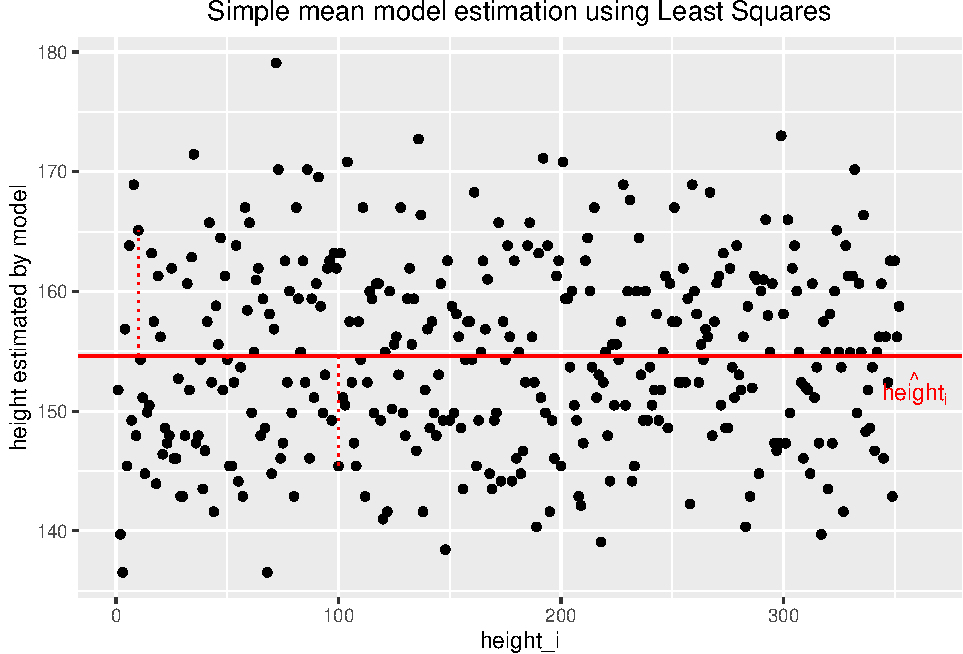
\includegraphics[keepaspectratio]{bookdown-demo_files/figure-latex/unnamed-chunk-15-1.pdf}}

Above, the heights are plotted against the index of the observation.
The variability of heights around the regression line (constant in this case) seems to
stay constant, which is a good sign. We will call this \textbf{homoscedasticity} later.
The dashed vertical red lines show two residuals, the difference between the actual height
and the estimated height. The model-estimated heights (\(\widehat{heights_i}\))
are all identical and nothing but the mean of all heights.

Peter Westfall explains in his excellent book a conditional distribution
approach to regression. I highly recommend reading the first chapters.

What does this mean in this context?

\section{Exercises}\label{exercises}

\subsection{{[}E{]} Exercise 1}\label{exercise1_Intro}

Use the \href{https://www.bfs.admin.ch/asset/de/30305714}{Swiss body heights} data to
determine
- the 95\% ``Vertrauensintervall'' for \(\mu\) and
- calculate the standard deviation of the heights from \(21,873\) Swiss people.

\subsection{{[}E{]} Exercise 2}\label{exercise2_Intro}

Why do we not need a hypothesis test to know that the population mean of body heights is not zero?
Give 2 reasons.

\subsection{{[}M{]} Exercise 3}\label{exercise3_Intro}

Verify analytically that the \texttt{Residual\ standard\ error} is identical with
the sample standard deviation of the heights.

\subsection{{[}M{]} Exercise 4}\label{exercise4_Intro}

Repeat the estimation of the simple model using a different data set about
\href{https://stat.ethz.ch/R-manual/R-devel/library/datasets/html/ChickWeight.html}{chicken weights},
which is included in R.

\begin{itemize}
\tightlist
\item
  Set useful priors for the mean and standard deviation of the model
  for the Baysian and the frequentist version considering
  your a priori knowledge about chicken weights.
\end{itemize}

\section{Addendum}\label{addendum}

\subsection{The bivariate normal distribution}\label{bivariate_normal}

As a refresher, you can look into the old QM1 script and read the
chapter ``4.7 Gemeinsame Verteilungen''.
Maybe \href{https://www.youtube.com/watch?v=SP2GKq8xJ5I&ab_channel=StatisticsNinja}{this video}
also helps.

The bivariate normal distribution is a generalization of the normal distribution to two dimensions.
Now, we look at the distribution of two random variables \(X\) and \(Y\) \textbf{at the same time}.

Instead of one Gaussian bell curve, we have a
\href{https://en.wikipedia.org/wiki/Multivariate_normal_distribution\#/media/File:Multivariate_Gaussian.png}{3D bell curve}.
This curve defines how plausible different combinations of \(X\) and \(Y\) are.

Single points (like (3,6)) still have probability zero, because now the \textbf{volume} over a single point
(\(x\), \(y\)) is zero. The probability of a certain area is now the \textbf{volume} under the
curve compared to the \textbf{area} under the density curve in the one-dimensional case.

\textbf{Example}: The following plot shows the density of a bivariate normal distribution of
two variables \(X\) and \(Y\)
with \(\mu_X = 0\), \(\mu_Y = 0\), \(\sigma_X = 1\), \(\sigma_Y = 1\) and \(\rho = \frac{2}{3}\).

Below is the correlation matrix of the bivariate normal distribution.

\begin{verbatim}
##           [,1]      [,2]
## [1,] 1.0000000 0.6666667
## [2,] 0.6666667 1.0000000
\end{verbatim}

\pandocbounded{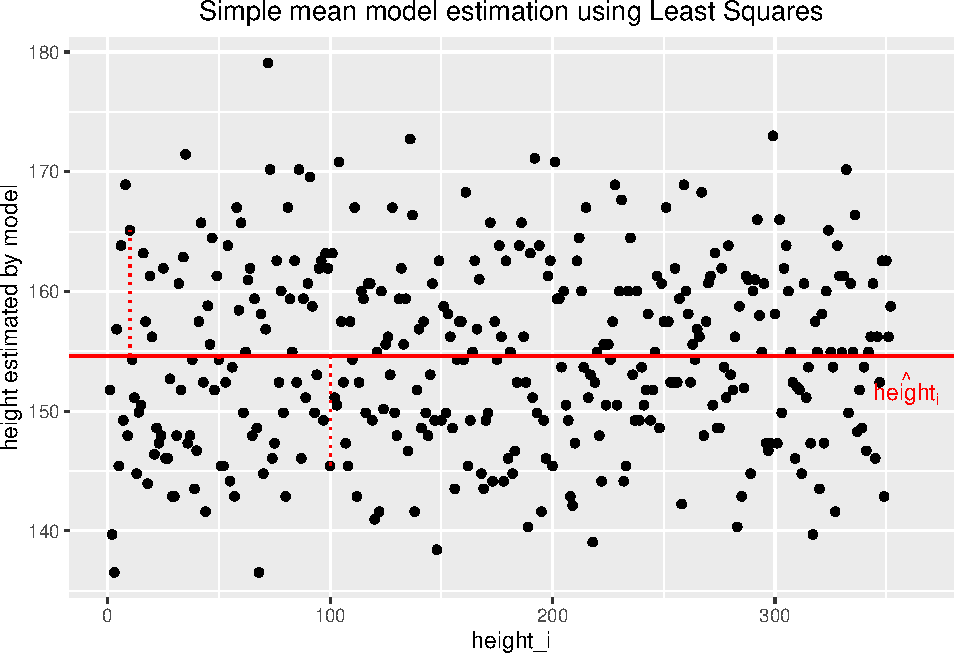
\includegraphics[keepaspectratio]{bookdown-demo_files/figure-latex/unnamed-chunk-16-1.pdf}}

If you move the plot around with your mouse, you see that there is a positive
correlation between \(X\) and \(Y\) (\(\rho = \frac{2}{3}\)). This means that if \(X\) is
above its mean, \(Y\) is also more likely to be above its mean.
The variances of \(X\) and \(Y\) are both \(1\). That means, that if you cut
through the plot in \(X=0\) or \(Y=0\), you see the same form of normal distribution.
If you look at if from above, we have hihglighted the section on the surface
over the area \(X \in [0.5, 2]\) and \(Y \in [0.5, 2]\). The volume over this area
under the density curve is the probability of this area: \(P(X \in [0.5, 2] \text{ and } Y \in [0.5, 2])\)

\chapter{Simple Linear Regression}\label{simple-linear-regression}

\section{Simple Linear Regression in the Bayesian Framework}\label{simple-linear-regression-in-the-bayesian-framework}

We will now add one covariate/explanatory variable to the model.
Refer to \href{https://civil.colorado.edu/~balajir/CVEN6833/bayes-resources/RM-StatRethink-Bayes.pdf}{Statistical Rethinking}
``4.4 Linear prediction'' or ``4.4 Adding a predictor'' as it's called in the online version of the book.

So far, our ``regression'' did not do much to be honest. The mean of a list of values
was already calculated in the \href{https://jdegenfellner.github.io/Script_QM1_ZHAW/descriptive_stats.html}{descriptive statistics section}
before and we have mentioned how great this statistic is as measure of location and where its weaknesses are.

Now, we want to model how body height and weight are related.
Formally, one wants to \emph{predict} body heights from body weights.

Here and in the frequentist framework, we will see that it is \textbf{not the same}
problem (and therefore results in a different statistical model)
\textbf{to predict body weights from body heights or vice versa}.

The word ``predictor'' is important here. It is a technical term
and describes a variable that we know (in our case weight) and with
which we want to ``guess as good as possible'' the value of the
dependent variable (in our case height).

We \textbf{always} visualize the data first to improve our understanding.

\begin{Shaded}
\begin{Highlighting}[]
\FunctionTok{plot}\NormalTok{(d2}\SpecialCharTok{$}\NormalTok{height }\SpecialCharTok{\textasciitilde{}}\NormalTok{ d2}\SpecialCharTok{$}\NormalTok{weight)}
\end{Highlighting}
\end{Shaded}

\pandocbounded{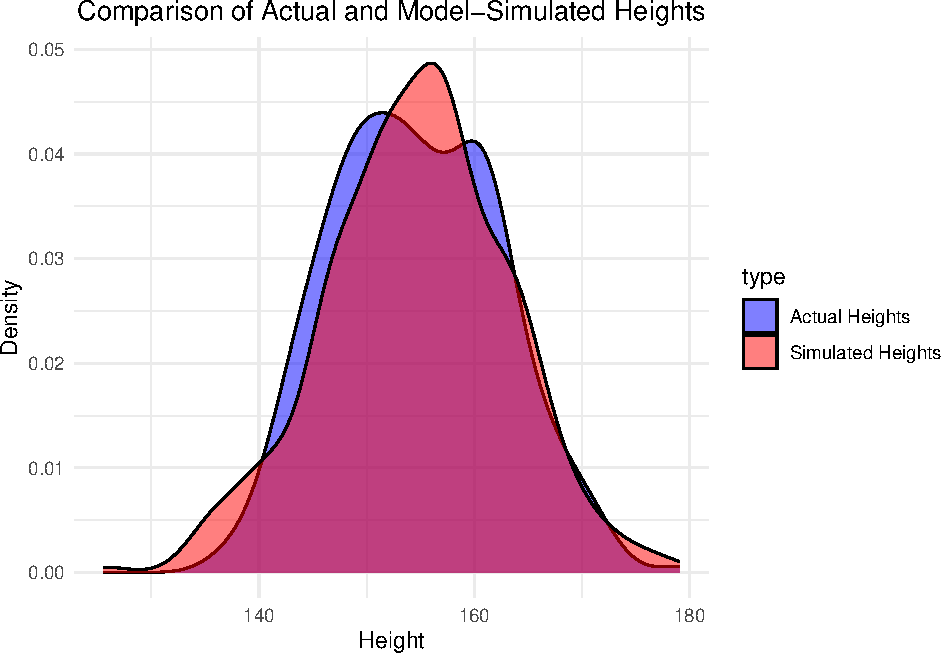
\includegraphics[keepaspectratio]{bookdown-demo_files/figure-latex/unnamed-chunk-17-1.pdf}}

The scatterplot indicates a linear relationship between the two variables.
The higher the weight, the higher the height; with some deviations of course.
This relationsip is neither causal, not deterministic.

\begin{itemize}
\tightlist
\item
  It is not causal since an increase in weight does not
  necessarily lead to an increase in height, especially in grown-ups.
\item
  It is not deterministic since there are deviations from the line.
  It if was deterministic, we would not need statistical modeling.
\end{itemize}

For simpler notation, we will call \texttt{d2\$weight} \(x\). \(\bar{x}\)
is the mean of \(x\).

\subsection{Model definition}\label{model-definition}

Let's write down our \textbf{model} (again with the Swiss population prior mean):

\begin{eqnarray*}
h_i &\sim& \text{Normal}(\mu_i, \sigma)\\
\mu_i &\sim& \alpha + \beta (x_i - \bar{x})\\
\alpha &\sim& \text{Normal}(171.1, 20)\\
\beta &\sim& \text{Normal}(0, 10)\\
\sigma &\sim& \text{Uniform}(0, 50)
\end{eqnarray*}

Visualization of the \textbf{model structure}:

\begin{verbatim}
## file:////private/var/folders/pm/jd6n6gj10371_bml1gh8sc5w0000gn/T/Rtmpl22xBb/file371b37e5a79f/widget371b465fd464.html screenshot completed
\end{verbatim}

\pandocbounded{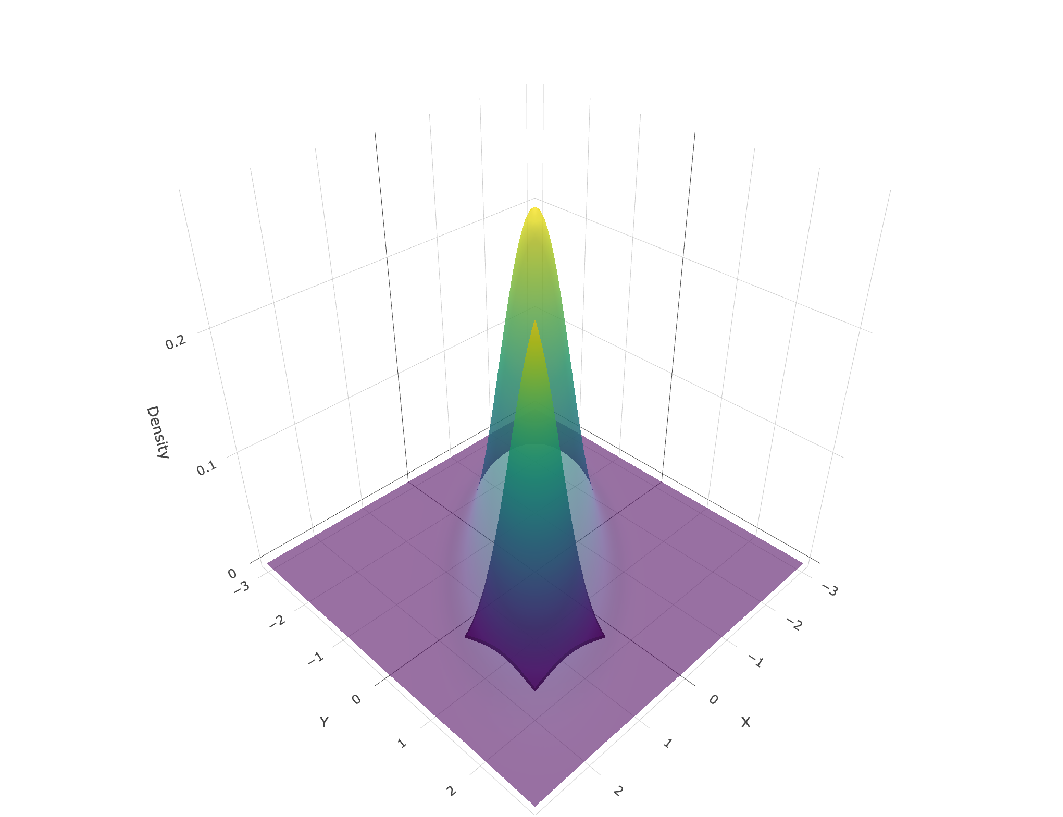
\includegraphics[keepaspectratio]{bookdown-demo_files/figure-latex/unnamed-chunk-18-1.pdf}}

There are now additional lines for the priors of \(\alpha\) and \(\beta\).
The model structure also shows the way to simulate from the prior.
One starts at the top and ends up with the heights.

\begin{itemize}
\tightlist
\item
  \(h_i\) is the height of the \(i\)-th person and we assume it is normally distributed.
\item
  \(\mu_i\) is the mean of the height of the \(i\)-th person and we
  assume it is normally distributed. Compared to the intercept model,
  a different mean is assumed for each person. \textbf{The mean \(\mu_i\) is linearly
  dependent on the weight} of the \(i\)-th person (second line).
\item
  \(\alpha\) is the intercept and we use the same prior as before.
\item
  \(\beta\) is the slope of the line and we use the normal distribution as prior for it,
  hence it can be positive or negative and how plausible each value is, is
  determined by that specific normal distribution. Note, that we could
  easily adapt the distribtion to any distribution we like.
\item
  The prior for \(\sigma\) is unchanged.
\item
  \(x_i - \bar{x}\) is the deviation of the weight from the mean weight, thereby \textbf{we
  center} the weight variable. This is a common practice in regression analysis.
\end{itemize}

The linear model is quite popular in applied statistics and one
reason is probably the rather straightforward interpretation of the coefficients.

\subsection{Priors}\label{priors}

We want to plot our priors to get a feeling what
the model would predict without seeing the data.
This is a kind of ``sanity check'' to see if the priors are reasonable.

\begin{Shaded}
\begin{Highlighting}[]
\FunctionTok{set.seed}\NormalTok{(}\DecValTok{2971}\NormalTok{)}
\NormalTok{N }\OtherTok{\textless{}{-}} \DecValTok{100}  \CommentTok{\# 100 lines}
\NormalTok{a }\OtherTok{\textless{}{-}} \FunctionTok{rnorm}\NormalTok{(N, }\FloatTok{171.1}\NormalTok{, }\DecValTok{20}\NormalTok{)}
\NormalTok{b }\OtherTok{\textless{}{-}} \FunctionTok{rnorm}\NormalTok{(N, }\DecValTok{0}\NormalTok{, }\DecValTok{10}\NormalTok{)}

\CommentTok{\# Assume d2$weight is defined, e.g., using some dataset or simulation}
\NormalTok{xbar }\OtherTok{\textless{}{-}} \FunctionTok{mean}\NormalTok{(d2}\SpecialCharTok{$}\NormalTok{weight)}

\FunctionTok{plot}\NormalTok{(}\ConstantTok{NULL}\NormalTok{, }\AttributeTok{xlim =} \FunctionTok{range}\NormalTok{(d2}\SpecialCharTok{$}\NormalTok{weight), }\AttributeTok{ylim =} \FunctionTok{c}\NormalTok{(}\SpecialCharTok{{-}}\DecValTok{100}\NormalTok{, }\DecValTok{400}\NormalTok{),}
     \AttributeTok{xlab =} \StringTok{"weight"}\NormalTok{, }\AttributeTok{ylab =} \StringTok{"height"}\NormalTok{)}
\FunctionTok{abline}\NormalTok{(}\AttributeTok{h =} \DecValTok{0}\NormalTok{, }\AttributeTok{lty =} \DecValTok{2}\NormalTok{)  }\CommentTok{\# horizontal line at 0}
\FunctionTok{abline}\NormalTok{(}\AttributeTok{h =} \DecValTok{272}\NormalTok{, }\AttributeTok{lty =} \DecValTok{1}\NormalTok{, }\AttributeTok{lwd =} \FloatTok{0.5}\NormalTok{)  }\CommentTok{\# horizontal line at 272}
\FunctionTok{mtext}\NormalTok{(}\StringTok{"b \textasciitilde{} dnorm(0, 10)"}\NormalTok{)}

\CommentTok{\# Overlay the 100 lines}
\ControlFlowTok{for}\NormalTok{ (i }\ControlFlowTok{in} \DecValTok{1}\SpecialCharTok{:}\NormalTok{N) \{}
  \FunctionTok{curve}\NormalTok{(a[i] }\SpecialCharTok{+}\NormalTok{ b[i] }\SpecialCharTok{*}\NormalTok{ (x }\SpecialCharTok{{-}}\NormalTok{ xbar),}
        \AttributeTok{from =} \FunctionTok{min}\NormalTok{(d2}\SpecialCharTok{$}\NormalTok{weight), }\AttributeTok{to =} \FunctionTok{max}\NormalTok{(d2}\SpecialCharTok{$}\NormalTok{weight),}
        \AttributeTok{add =} \ConstantTok{TRUE}\NormalTok{, }\AttributeTok{col =} \FunctionTok{col.alpha}\NormalTok{(}\StringTok{"black"}\NormalTok{, }\FloatTok{0.2}\NormalTok{))}
\NormalTok{\}}
\end{Highlighting}
\end{Shaded}

\pandocbounded{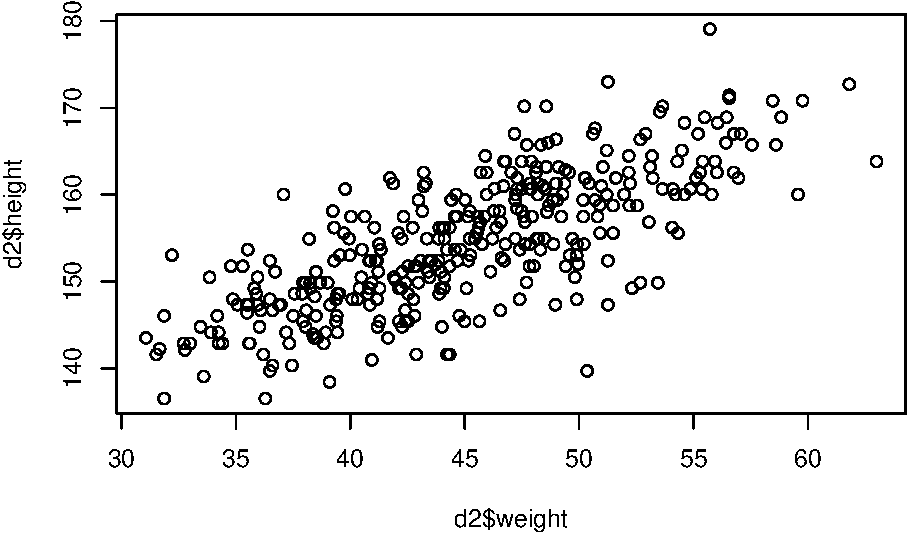
\includegraphics[keepaspectratio]{bookdown-demo_files/figure-latex/unnamed-chunk-19-1.pdf}}

This relationship seems rather non-restrictive. According to our priors,
one could see very steeply rising or falling lines. We could at least make
the priors for the slope (\(\beta\)) non-negative. One possibility to do this
is to use a \href{https://en.wikipedia.org/wiki/Log-normal_distribution}{log-normal distribution}
for the prior of \(\beta\) which can only take non-negative values.

\[ \beta \sim \text{Log-Normal}(0, 1) \]

Lets plot the priors again.

\begin{Shaded}
\begin{Highlighting}[]
\FunctionTok{set.seed}\NormalTok{(}\DecValTok{2971}\NormalTok{)}
\NormalTok{N }\OtherTok{\textless{}{-}} \DecValTok{100}  \CommentTok{\# 100 lines}
\NormalTok{a }\OtherTok{\textless{}{-}} \FunctionTok{rnorm}\NormalTok{(N, }\FloatTok{171.1}\NormalTok{, }\DecValTok{20}\NormalTok{)}
\NormalTok{b }\OtherTok{\textless{}{-}} \FunctionTok{rlnorm}\NormalTok{(N, }\DecValTok{0}\NormalTok{, }\DecValTok{1}\NormalTok{)}

\CommentTok{\# Assume d2$weight is defined, e.g., using some dataset or simulation}
\NormalTok{xbar }\OtherTok{\textless{}{-}} \FunctionTok{mean}\NormalTok{(d2}\SpecialCharTok{$}\NormalTok{weight)}

\FunctionTok{plot}\NormalTok{(}\ConstantTok{NULL}\NormalTok{, }\AttributeTok{xlim =} \FunctionTok{range}\NormalTok{(d2}\SpecialCharTok{$}\NormalTok{weight), }\AttributeTok{ylim =} \FunctionTok{c}\NormalTok{(}\SpecialCharTok{{-}}\DecValTok{100}\NormalTok{, }\DecValTok{400}\NormalTok{),}
     \AttributeTok{xlab =} \StringTok{"weight"}\NormalTok{, }\AttributeTok{ylab =} \StringTok{"height"}\NormalTok{)}
\FunctionTok{abline}\NormalTok{(}\AttributeTok{h =} \DecValTok{0}\NormalTok{, }\AttributeTok{lty =} \DecValTok{2}\NormalTok{)  }\CommentTok{\# horizontal line at 0}
\FunctionTok{abline}\NormalTok{(}\AttributeTok{h =} \DecValTok{272}\NormalTok{, }\AttributeTok{lty =} \DecValTok{1}\NormalTok{, }\AttributeTok{lwd =} \FloatTok{0.5}\NormalTok{)  }\CommentTok{\# horizontal line at 272}
\FunctionTok{mtext}\NormalTok{(}\StringTok{"b \textasciitilde{} dlnorm(0, 1)"}\NormalTok{)}

\CommentTok{\# Overlay the 100 lines}
\ControlFlowTok{for}\NormalTok{ (i }\ControlFlowTok{in} \DecValTok{1}\SpecialCharTok{:}\NormalTok{N) \{}
  \FunctionTok{curve}\NormalTok{(a[i] }\SpecialCharTok{+}\NormalTok{ b[i] }\SpecialCharTok{*}\NormalTok{ (x }\SpecialCharTok{{-}}\NormalTok{ xbar),}
        \AttributeTok{from =} \FunctionTok{min}\NormalTok{(d2}\SpecialCharTok{$}\NormalTok{weight), }\AttributeTok{to =} \FunctionTok{max}\NormalTok{(d2}\SpecialCharTok{$}\NormalTok{weight),}
        \AttributeTok{add =} \ConstantTok{TRUE}\NormalTok{, }\AttributeTok{col =} \FunctionTok{col.alpha}\NormalTok{(}\StringTok{"black"}\NormalTok{, }\FloatTok{0.2}\NormalTok{))}
\NormalTok{\}}
\end{Highlighting}
\end{Shaded}

\pandocbounded{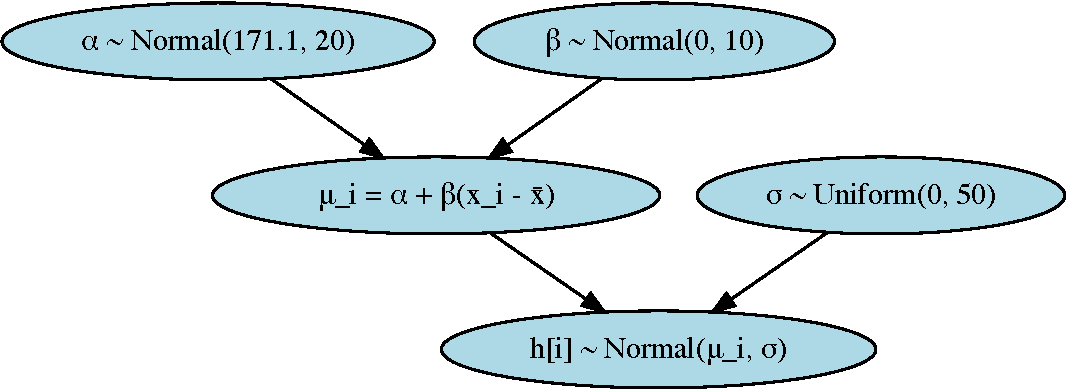
\includegraphics[keepaspectratio]{bookdown-demo_files/figure-latex/unnamed-chunk-20-1.pdf}}

This seems definitely more realistic.

\subsection{Fit model}\label{fit-model}

Now, let's \textbf{estimate the posterior/fit the model} as before:

\begin{Shaded}
\begin{Highlighting}[]
\CommentTok{\# load data again, since it\textquotesingle{}s a long way back}
\FunctionTok{library}\NormalTok{(rethinking)}
\FunctionTok{data}\NormalTok{(Howell1)}
\NormalTok{d }\OtherTok{\textless{}{-}}\NormalTok{ Howell1}
\NormalTok{d2 }\OtherTok{\textless{}{-}}\NormalTok{ d[d}\SpecialCharTok{$}\NormalTok{age }\SpecialCharTok{\textgreater{}=} \DecValTok{18}\NormalTok{, ]}
\NormalTok{xbar }\OtherTok{\textless{}{-}} \FunctionTok{mean}\NormalTok{(d2}\SpecialCharTok{$}\NormalTok{weight)}
\CommentTok{\# fit model}
\NormalTok{mod }\OtherTok{\textless{}{-}} \FunctionTok{quap}\NormalTok{(}
    \FunctionTok{alist}\NormalTok{(}
\NormalTok{        height }\SpecialCharTok{\textasciitilde{}} \FunctionTok{dnorm}\NormalTok{(mu, sigma),}
\NormalTok{        mu }\OtherTok{\textless{}{-}}\NormalTok{ a }\SpecialCharTok{+}\NormalTok{ b }\SpecialCharTok{*}\NormalTok{ (weight }\SpecialCharTok{{-}}\NormalTok{ xbar),}
\NormalTok{        a }\SpecialCharTok{\textasciitilde{}} \FunctionTok{dnorm}\NormalTok{(}\FloatTok{171.1}\NormalTok{, }\DecValTok{100}\NormalTok{),}
\NormalTok{        b }\SpecialCharTok{\textasciitilde{}} \FunctionTok{dnorm}\NormalTok{(}\DecValTok{0}\NormalTok{, }\DecValTok{10}\NormalTok{),}
\NormalTok{        sigma }\SpecialCharTok{\textasciitilde{}} \FunctionTok{dunif}\NormalTok{(}\DecValTok{0}\NormalTok{, }\DecValTok{50}\NormalTok{)}
\NormalTok{    ) ,}
\AttributeTok{data =}\NormalTok{ d2)}
\end{Highlighting}
\end{Shaded}

Let's look at the \textbf{marginal distributions} of the parameters:

\begin{Shaded}
\begin{Highlighting}[]
\FunctionTok{precis}\NormalTok{(mod)}
\end{Highlighting}
\end{Shaded}

\begin{verbatim}
##              mean         sd        5.5%       94.5%
## a     154.5972120 0.27033045 154.1651717 155.0292523
## b       0.9050131 0.04192754   0.8380048   0.9720214
## sigma   5.0718673 0.19115323   4.7663675   5.3773671
\end{verbatim}

The analysis yields estimates for all our parameters of the model: \(\alpha\),
\(\beta\) and \(\sigma\). The estimates are the mean of the posterior distribution.

See \hyperref[exercise2_simpl_lin_reg]{exercise 2}.

\textbf{Interpretation of \(\beta\)}:
The mean of the posterior distribution of \(\beta\) is 0.9. A person with a weight
of 1 kg more weight can be expected to be 0.9 cm taller. A 96\% credible interval
for this estimate is \([0.83, 0.97]\). We can be quite sure that the slope is
positive.

It might also be interesting to insept the variance-covariance matrix,
respectively the correlation between the parameters as we did before
in the intercept model.

\begin{Shaded}
\begin{Highlighting}[]
\FunctionTok{diag}\NormalTok{(}\FunctionTok{vcov}\NormalTok{(mod))}
\end{Highlighting}
\end{Shaded}

\begin{verbatim}
##           a           b       sigma 
## 0.073078550 0.001757918 0.036539558
\end{verbatim}

\begin{Shaded}
\begin{Highlighting}[]
\FunctionTok{cov2cor}\NormalTok{(}\FunctionTok{vcov}\NormalTok{(mod))}
\end{Highlighting}
\end{Shaded}

\begin{verbatim}
##                   a             b         sigma
## a      1.000000e+00 -9.591866e-10  3.330963e-05
## b     -9.591866e-10  1.000000e+00 -2.879607e-05
## sigma  3.330963e-05 -2.879607e-05  1.000000e+00
\end{verbatim}

As we can see the correlations are near zero. Compare to the graphical
display of the model structure. There is no connection.

\subsection{Result}\label{result}

\textbf{Graphical end result} of fitting the model:

\begin{Shaded}
\begin{Highlighting}[]
\FunctionTok{plot}\NormalTok{(d2}\SpecialCharTok{$}\NormalTok{height }\SpecialCharTok{\textasciitilde{}}\NormalTok{ d2}\SpecialCharTok{$}\NormalTok{weight, }\AttributeTok{col =}\NormalTok{ rangi2)}
\NormalTok{post }\OtherTok{\textless{}{-}} \FunctionTok{extract.samples}\NormalTok{(mod)}
\NormalTok{a\_quap }\OtherTok{\textless{}{-}} \FunctionTok{mean}\NormalTok{(post}\SpecialCharTok{$}\NormalTok{a)}
\NormalTok{b\_quap }\OtherTok{\textless{}{-}} \FunctionTok{mean}\NormalTok{(post}\SpecialCharTok{$}\NormalTok{b)}
\FunctionTok{curve}\NormalTok{(a\_quap }\SpecialCharTok{+}\NormalTok{ b\_quap }\SpecialCharTok{*}\NormalTok{ (x }\SpecialCharTok{{-}}\NormalTok{ xbar), }\AttributeTok{add =} \ConstantTok{TRUE}\NormalTok{)}
\end{Highlighting}
\end{Shaded}

\pandocbounded{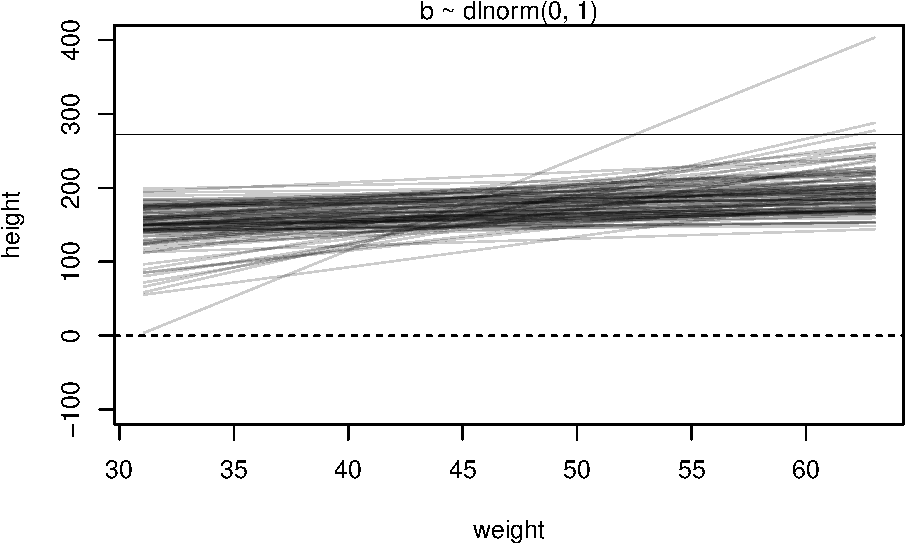
\includegraphics[keepaspectratio]{bookdown-demo_files/figure-latex/unnamed-chunk-24-1.pdf}}

\subsection{Credible bands}\label{credible-bands}

We could draw again and again from the posterior distribution
and calculate the means like above. Plotting the regression lines
with the respective parameters \(\alpha\), \(\beta\) would indicate
the variability of the estimates.

\begin{Shaded}
\begin{Highlighting}[]
\CommentTok{\# Define a sequence of weights for predictions}
\NormalTok{weight.seq }\OtherTok{\textless{}{-}} \FunctionTok{seq}\NormalTok{(}\AttributeTok{from =} \DecValTok{25}\NormalTok{, }\AttributeTok{to =} \DecValTok{70}\NormalTok{, }\AttributeTok{by =} \DecValTok{1}\NormalTok{)}

\CommentTok{\# Use the model to compute mu for each weight}
\NormalTok{mu }\OtherTok{\textless{}{-}} \FunctionTok{link}\NormalTok{(mod, }\AttributeTok{data =} \FunctionTok{data.frame}\NormalTok{(}\AttributeTok{weight =}\NormalTok{ weight.seq))}
\FunctionTok{str}\NormalTok{(mu)}
\end{Highlighting}
\end{Shaded}

\begin{verbatim}
##  num [1:1000, 1:46] 138 136 137 136 137 ...
\end{verbatim}

\begin{Shaded}
\begin{Highlighting}[]
\CommentTok{\# Visualize the distribution of mu values}
\FunctionTok{plot}\NormalTok{(height }\SpecialCharTok{\textasciitilde{}}\NormalTok{ weight, d2, }\AttributeTok{type =} \StringTok{"n"}\NormalTok{)  }\CommentTok{\# Hide raw data with type = "n"}

\CommentTok{\# Loop over samples and plot each mu value}
\ControlFlowTok{for}\NormalTok{ (i }\ControlFlowTok{in} \DecValTok{1}\SpecialCharTok{:}\DecValTok{100}\NormalTok{) \{}
  \FunctionTok{points}\NormalTok{(weight.seq, mu[i, ], }\AttributeTok{pch =} \DecValTok{16}\NormalTok{, }\AttributeTok{col =} \FunctionTok{col.alpha}\NormalTok{(rangi2, }\FloatTok{0.1}\NormalTok{))}
\NormalTok{\}}
\end{Highlighting}
\end{Shaded}

\pandocbounded{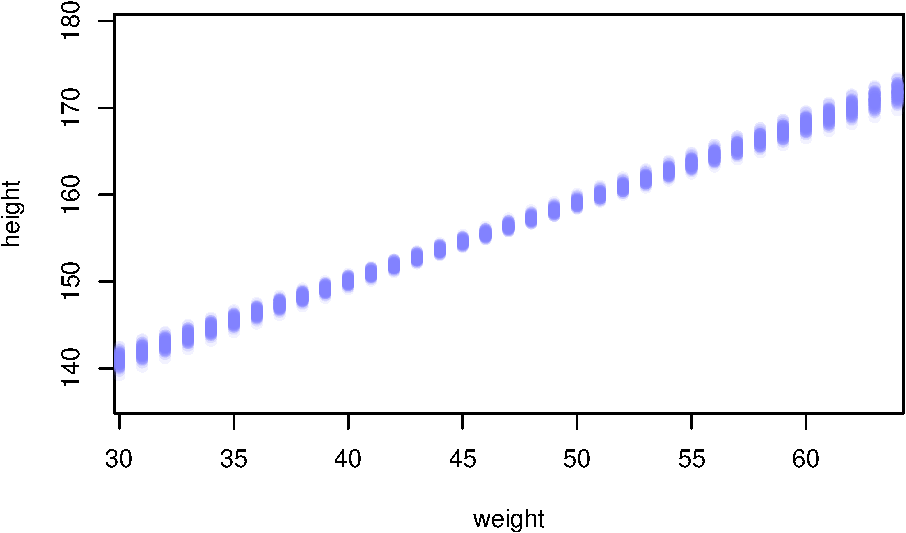
\includegraphics[keepaspectratio]{bookdown-demo_files/figure-latex/unnamed-chunk-25-1.pdf}}

The \texttt{link} function fixes the weight at the values in \texttt{weight.seq} and
draws samples from the posterior distribution of the parameters. We will do
the analog thing in the frequentist framework.

We can also draw a nice shade for the regression line:

\begin{Shaded}
\begin{Highlighting}[]
\CommentTok{\# Summarize the distribution of mu}
\NormalTok{mu.mean }\OtherTok{\textless{}{-}} \FunctionTok{apply}\NormalTok{(mu, }\DecValTok{2}\NormalTok{, mean)}
\NormalTok{mu.PI }\OtherTok{\textless{}{-}} \FunctionTok{apply}\NormalTok{(mu, }\DecValTok{2}\NormalTok{, PI, }\AttributeTok{prob =} \FloatTok{0.89}\NormalTok{)}
\FunctionTok{plot}\NormalTok{(height }\SpecialCharTok{\textasciitilde{}}\NormalTok{ weight, d2, }\AttributeTok{col =} \FunctionTok{col.alpha}\NormalTok{(rangi2, }\FloatTok{0.5}\NormalTok{))}
\FunctionTok{lines}\NormalTok{(weight.seq, mu.mean)}
\FunctionTok{shade}\NormalTok{(mu.PI, weight.seq)}
\end{Highlighting}
\end{Shaded}

\pandocbounded{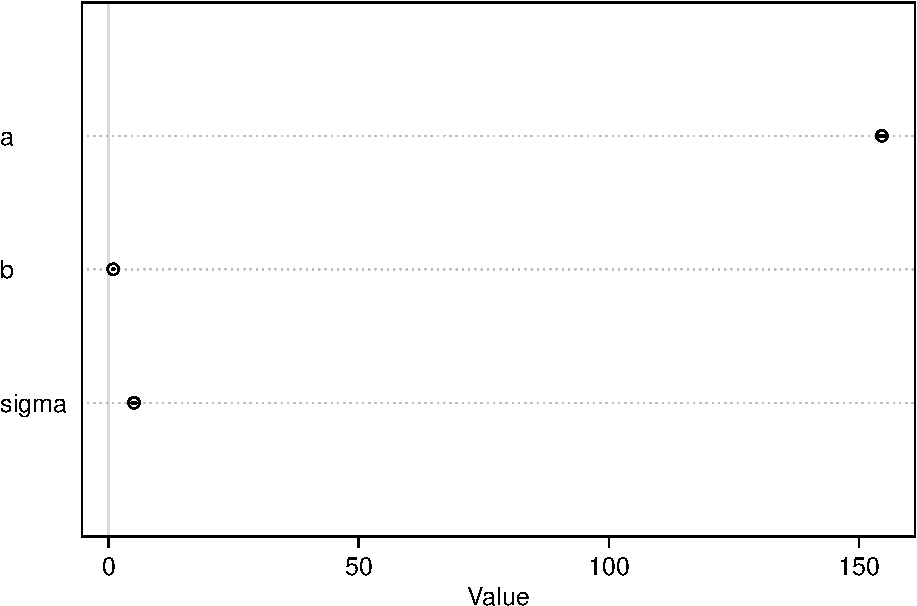
\includegraphics[keepaspectratio]{bookdown-demo_files/figure-latex/unnamed-chunk-26-1.pdf}}

As we can see, we are pretty sure about the mean of height which
we wanted to model in the first place.
Mean modeling is one thing, individual prediction is another.
Given a certain weight of a person, what is the height of the same person?
The first line in the model definition (\(height_i \sim Normal(\mu_i, \sigma)\))
tells us that a person's weight is distributed \emph{around} the mean
(which linearly depends on weight) and is not necessary the mean itself.

To get to an \textbf{individual prediction}, we need to consider the uncertainty
of the parameter estimation \emph{and} the uncertainty from the Gaussian distribution
around the mean (at a certain weight). We do this with \texttt{sim}.

\begin{Shaded}
\begin{Highlighting}[]
\CommentTok{\# Simulate heights from the posterior}
\NormalTok{sim.height }\OtherTok{\textless{}{-}} \FunctionTok{sim}\NormalTok{(mod, }\AttributeTok{data =} \FunctionTok{list}\NormalTok{(}\AttributeTok{weight =}\NormalTok{ weight.seq))}
\FunctionTok{str}\NormalTok{(sim.height)}
\end{Highlighting}
\end{Shaded}

\begin{verbatim}
##  num [1:1000, 1:46] 138 130 130 147 136 ...
\end{verbatim}

\begin{Shaded}
\begin{Highlighting}[]
\CommentTok{\# Compute the 89\% prediction interval for simulated heights}
\NormalTok{height.PI }\OtherTok{\textless{}{-}} \FunctionTok{apply}\NormalTok{(sim.height, }\DecValTok{2}\NormalTok{, PI, }\AttributeTok{prob =} \FloatTok{0.89}\NormalTok{)}

\CommentTok{\# Plot the raw data}
\FunctionTok{plot}\NormalTok{(height }\SpecialCharTok{\textasciitilde{}}\NormalTok{ weight, d2, }\AttributeTok{col =} \FunctionTok{col.alpha}\NormalTok{(rangi2, }\FloatTok{0.5}\NormalTok{))}

\CommentTok{\# Draw MAP (mean a posteriori) line}
\FunctionTok{lines}\NormalTok{(weight.seq, mu.mean)}

\CommentTok{\# Draw HPDI (highest posterior density interval) region for mu}
\FunctionTok{shade}\NormalTok{(mu.PI, weight.seq)}

\CommentTok{\# Draw PI (prediction interval) region for simulated heights}
\FunctionTok{shade}\NormalTok{(height.PI, weight.seq)}
\end{Highlighting}
\end{Shaded}

\pandocbounded{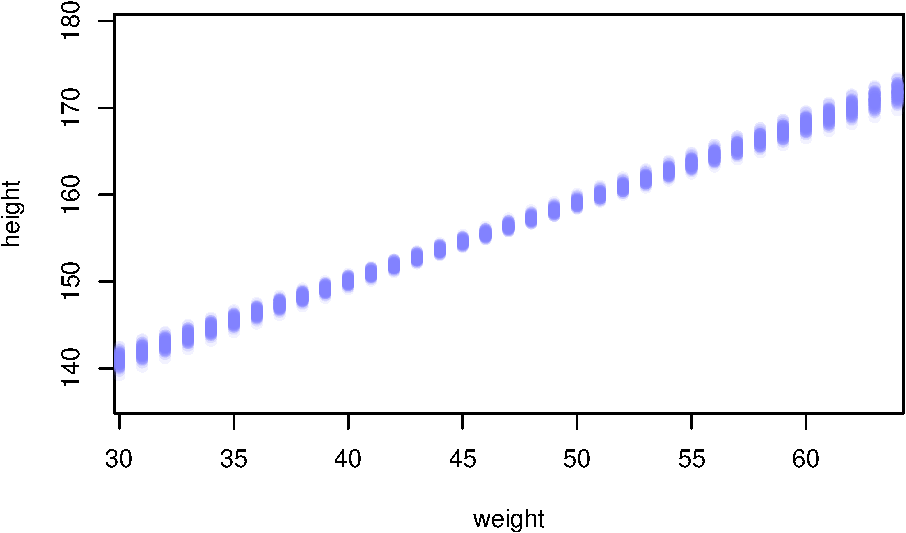
\includegraphics[keepaspectratio]{bookdown-demo_files/figure-latex/unnamed-chunk-27-1.pdf}}

The lighter and wider shaded region is where the model expects to find 89\%
of the heights of a person with a certain weight.

This part is sometimes a bit desillusioning when seen for the first time:
Draw a horizontal line at 150 cm and see how many weights (according to
the individual prediction) are compatible with this height. Weights
from 30 to 50 kg are compatible with this height according to the
89\% prediction interval. The higher the credibility, the wider the interval,
the wider the range of compatible weights (more than 60\% of the weight-range).

\begin{Shaded}
\begin{Highlighting}[]
\NormalTok{(}\DecValTok{50} \SpecialCharTok{{-}} \DecValTok{30}\NormalTok{) }\SpecialCharTok{/}\NormalTok{ (}\FunctionTok{range}\NormalTok{(d2}\SpecialCharTok{$}\NormalTok{weight)[}\DecValTok{2}\NormalTok{] }\SpecialCharTok{{-}} \FunctionTok{range}\NormalTok{(d2}\SpecialCharTok{$}\NormalTok{weight)[}\DecValTok{1}\NormalTok{])}
\end{Highlighting}
\end{Shaded}

\begin{verbatim}
## [1] 0.6265362
\end{verbatim}

\subsection{Summary}\label{summary}

\begin{itemize}
\tightlist
\item
  We have added a covariate (weight) to the simple mean model to predict height.
\item
  We have centered the weight variable.
\item
  We have defined and refined priors for the intercept and slope.
\item
  We have estimated the posterior distribution of the parameters using quadratic approximation with \texttt{quap}.
\item
  We have visualized the result.
\item
  We have created credible bands for mean and individual predictions.
\end{itemize}

\section{Simple Linear Regression in the Frequentist Framework}\label{simple-linear-regression-in-the-frequentist-framework}

We will now do the same analysis in the frequentist framework while introducing
some foundational theory along the way.
I recommend reading the first couple of chapters from \href{https://www.routledge.com/Understanding-Regression-Analysis-A-Conditional-Distribution-Approach/Westfall-Arias/p/book/9780367493516?srsltid=AfmBOore3O_Ciecl0TTkr9AjPIY1d6OmbQa7o7IAdKpTSkD8s9HkwzD4}{Westfall}.

\subsection{Model definition}\label{model-definition-1}

Our linear model is defined as:

\[ h_i = \beta_0 + \beta_1 x_i + \varepsilon_i \]

where

\begin{itemize}
\tightlist
\item
  \(\varepsilon_i\) is the error term with \(\varepsilon_i \sim N(0, \sigma), \forall i\)
\item
  \(\beta_0\) is the unknown but fixed intercept
\item
  \(\beta_1\) is the unknown but fixed slope
\end{itemize}

\subsubsection{\texorpdfstring{Model Assumptions of the Classical Regression Model (\href{https://www.routledge.com/Understanding-Regression-Analysis-A-Conditional-Distribution-Approach/Westfall-Arias/p/book/9780367493516?srsltid=AfmBOore3O_Ciecl0TTkr9AjPIY1d6OmbQa7o7IAdKpTSkD8s9HkwzD4}{Westfall}, 1.7):}{Model Assumptions of the Classical Regression Model (Westfall, 1.7):}}\label{model-assumptions-of-the-classical-regression-model-westfall-1.7}

The first and \textbf{most important assumption} is that the data are produced\\
probabilistically, which is specifically stated as
\[ Y|X = x \sim p(y|x)\]

What does this mean?

\begin{itemize}
\tightlist
\item
  \(Y|X = x\) is the random variable Y \textbf{conditional} on X being equal to x, i.e.~the
  distribution of \(Y\) if we know the value of \(X\) (in our example the weight in kg).
  \href{https://blogs.sas.com/content/iml/files/2015/09/GLM_normal_identity.png}{This} is a nice image of what is meant here.
\item
  \(p(y|x)\) is the distribution of potentially observable \(Y\) given \(X = x\).
  In our case above this was the normal distribution with mean \(\mu_i\) and variance \(\sigma\).
\end{itemize}

One always things about the so-called data
\href{https://en.wikipedia.org/wiki/Data_generating_process}{generating process}
(\href{https://www.routledge.com/Understanding-Regression-Analysis-A-Conditional-Distribution-Approach/Westfall-Arias/p/book/9780367493516?srsltid=AfmBOore3O_Ciecl0TTkr9AjPIY1d6OmbQa7o7IAdKpTSkD8s9HkwzD4}{Westfall}, 1.2).
How did the data come about? There is a process behind it and this process
is attempted to be modeled.

Further assumptions:

\begin{itemize}
\item
  Correct functional specification: The conditional mean function \(f(x) = \mathbb{E}(Y|X=x)\).
  In the case of the linear model, the assumption is \(\mathbb{E}(Y|X=x) = \alpha + \beta x\).
  The expectation of \(Y\) (height) depends linearly on \(x\) (weight).
\item
  The errors are homoscedastic (constant variance \(\sigma\)). This means the
  variances of all conditional distributions \(p(y|x)\) are constant (\(=\sigma^2\)).
\item
  Normality. For the classical linear regression model all the conditional
  distributions \(p(y|x)\) are normal distributions.
\item
  The errors are independent of each other.
  The potentially observable \(\varepsilon_i = Y_i - f(\mathbf{x_i}, \mathbf{\beta})\)
  is uncorrelated with \(\varepsilon_j = Y_j - f(\mathbf{x_j}, \mathbf{\beta})\) for
  \(i \neq j\).
\end{itemize}

These assumptions become clearer as we go along and should be checked
for every model we fit. They are not connected, they can all be true or false.
The question is not ``Are the assumptions met?'' since they never are exactly met.
The question is \textbf{how} ``badly'' the assumptions are violated?

Remember, \textbf{all models are wrong, but some are useful}.

In full, the classical linear regression model can be written as:

\[ Y_i|X_i = x_i \sim_{independent} N(\beta_0 + \beta_1 x_{i1} + \dots \beta_k x_{ik},\sigma^2)\]
for \(i = 1, \dots, n\).

\subsection{Fit the model}\label{fit-the-model}

Again, we fit the model using the least squares method.
One has to minimize the sum of squared differences between the true heights and
the model-predicted heights in order to find \(\beta_0\) and \(\beta_1\).

\[ SSE(\beta_0, \beta_1) = \sum_{i=1}^n (y_i - (\beta_0 + \beta_1 x_i))^2 \]

We omit the technical details and give the results for \(\beta_0\) and \(\beta_1\):

\[
\hat{\beta_0} = \bar{y} - (\hat{\beta_1} \bar{x}),
\]
\[
\hat{\beta_1} = \frac{\sum_{i=1}^n (x_i - \bar{x})(y_i - \bar{y})}{\sum_{i=1}^n (x_i - \bar{x})^2}.
\]

Let's use R again to solve the problem:

\begin{Shaded}
\begin{Highlighting}[]
\FunctionTok{library}\NormalTok{(rethinking)}
\FunctionTok{data}\NormalTok{(Howell1)}
\NormalTok{d }\OtherTok{\textless{}{-}}\NormalTok{ Howell1}
\NormalTok{d2 }\OtherTok{\textless{}{-}}\NormalTok{ d[d}\SpecialCharTok{$}\NormalTok{age }\SpecialCharTok{\textgreater{}=} \DecValTok{18}\NormalTok{, ]}
\NormalTok{mod }\OtherTok{\textless{}{-}} \FunctionTok{lm}\NormalTok{(height }\SpecialCharTok{\textasciitilde{}}\NormalTok{ weight, }\AttributeTok{data =}\NormalTok{ d2)}
\FunctionTok{summary}\NormalTok{(mod)}
\end{Highlighting}
\end{Shaded}

\begin{verbatim}
## 
## Call:
## lm(formula = height ~ weight, data = d2)
## 
## Residuals:
##      Min       1Q   Median       3Q      Max 
## -19.7464  -2.8835   0.0222   3.1424  14.7744 
## 
## Coefficients:
##              Estimate Std. Error t value Pr(>|t|)    
## (Intercept) 113.87939    1.91107   59.59   <2e-16 ***
## weight        0.90503    0.04205   21.52   <2e-16 ***
## ---
## Signif. codes:  0 '***' 0.001 '**' 0.01 '*' 0.05 '.' 0.1 ' ' 1
## 
## Residual standard error: 5.086 on 350 degrees of freedom
## Multiple R-squared:  0.5696, Adjusted R-squared:  0.5684 
## F-statistic: 463.3 on 1 and 350 DF,  p-value: < 2.2e-16
\end{verbatim}

\textbf{Interpretation of R-output}:

\begin{itemize}
\tightlist
\item
  \texttt{Call}: The model that was fitted.
\item
  \texttt{Residuals}: \(r_i = height_i - \widehat{height}_i\).
  Difference between true heights and model-predicted heights.
\item
  \texttt{Coefficients}: The estimated \(\beta_0\) and \(\beta_1\).

  \begin{itemize}
  \tightlist
  \item
    \texttt{Estimate}: The (least squares) estimated value of the coefficient.
  \item
    \texttt{Std.\ Error}: The standard error of the estimate.
  \item
    \texttt{t\ value}: The value of the \(t\)-statistic for the (Wald-) hypothesis test
    \(H_0: \beta_i = 0\).
  \item
    \texttt{Pr(\textgreater{}\textbar{}t\textbar{})}: The \(p\)-value of the hypothesis test.
  \end{itemize}
\item
  \texttt{Residual\ standard\ error}: The estimate of \(\sigma\)
  which is also a model parameter (as in the Bayesian framework).
\item
  \texttt{Multiple\ R-squared}: The proportion of the variance explained by the
  model (we will explain this below).
\item
  \texttt{Adjusted\ R-squared}: A corrected version of the \(R^2\) which takes into account
  the number of predictors in the model.
\item
  \texttt{F-statistic}: The value of the \(F\)-statistic for the hypothesis test:
  \(H_0: \beta_1 = \beta_2 = \dots = \beta_k = 0\). Note, the alternative
  hypotheses to this test is that \emph{any} of the \(\beta_i\) is not zero. If that Is
  the case, the model explains more than the mean model with just \(\beta_0\).
\end{itemize}

\subsection{ANOVA (Analysis of Variance)}\label{anova-analysis-of-variance}

A non-obvious and very useful finding is that the total variability in the data can be
\textbf{decomposed} (or \href{https://en.wiktionary.org/wiki/analysis}{analysed})
into two parts:

\begin{itemize}
\tightlist
\item
  The variability explained by the model (the regression line)
\item
  The variability not explained by the model (the residuals)
\end{itemize}

\[ \text{Total sum of squares} = \text{Regression sum of squares} + \text{Residual sum of squares} \]

\[ SST = SSR + SSE \]

\[ \sum (y_i - \bar{y})^2 = \sum (\hat{y}_i - \bar{y})^2 + \sum (y_i - \hat{y}_i)^2 \]

If you are interested in the details, check out \href{https://en.wikipedia.org/wiki/Explained_sum_of_squares\#Partitioning_in_the_general_ordinary_least_squares_model}{this}.

\href{https://www.youtube.com/watch?v=NxRTs7sXKAQ&ab_channel=365DataScience}{This video}
explains the concept nicely.

Let's visualize our regression result:

\begin{verbatim}
## `geom_smooth()` using formula = 'y ~ x'
\end{verbatim}

\pandocbounded{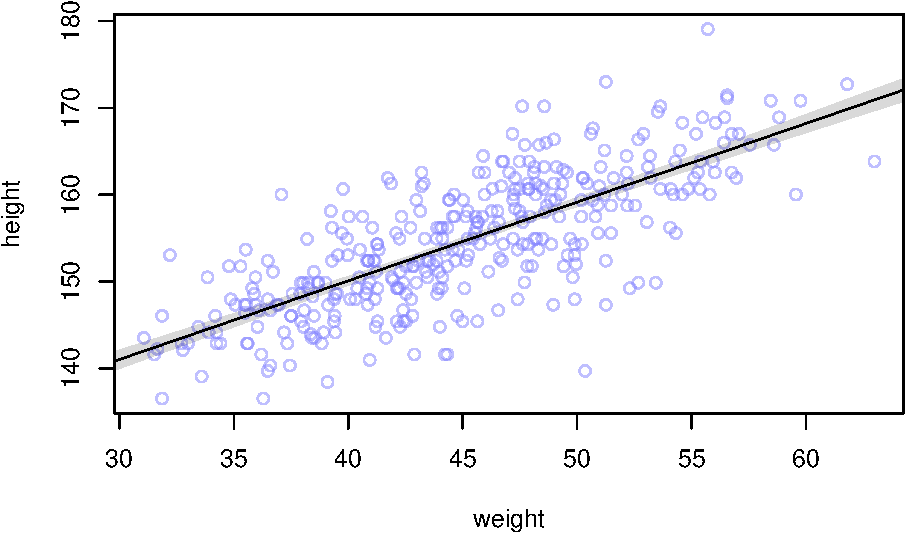
\includegraphics[keepaspectratio]{bookdown-demo_files/figure-latex/unnamed-chunk-30-1.pdf}}

\ldots\ldots. \textbf{TODOS}

\begin{itemize}
\tightlist
\item
  Conditional distribution approach
\item
  Not the same to predict X with Y or vice versa.
\item
  Analysis of Variance, R\^{}2
\item
  random X vs fixed X
\item
  separability interpretration using R\^{}2
\item
  check assumptions of model
\item
  interpret alpha and beta maybe using simulation
\end{itemize}

\section{Exercises}\label{exercises-1}

\subsection{Exercise 1}\label{exercise1_simpl_lin_reg}

In the model from above:

\begin{eqnarray*}
h_i &\sim& \text{Normal}(\mu_i, \sigma)\\
\mu_i &\sim& \alpha + \beta (x_i - \bar{x})\\
\alpha &\sim& \text{Normal}(171.1, 20)\\
\beta &\sim& \text{Normal}(0, 10)\\
\sigma &\sim& \text{Uniform}(0, 50)
\end{eqnarray*}

\begin{itemize}
\tightlist
\item
  What ist the expected height when \(x_i = \bar{x}\)?
\item
  What is the expected height when \(x_i\) changes by 1 unit?
\end{itemize}

\subsection{Exercise 2}\label{exercise2_simpl_lin_reg}

Look at the marginal distrubutions of the parameters in the Bayesian model.

\begin{itemize}
\tightlist
\item
  Plot the posterior distribution of all 3 parameters.
\item
  Include in the plot a 99\% credible interval (HDI).
\end{itemize}

\bibliography{book.bib,packages.bib}

\end{document}
